\documentclass[a4paper, fleqn]{article}
\usepackage{../header}

% Нумеруем только subsection
\renewcommand{\thesubsection}{\arabic{subsection}.}

\title{Математический Анализ 2, Коллоквиум \uppercase\expandafter{\romannumeral 2}}
\author{
    \normalsize
    % Добавь себя в список!
    % Имя фамилия          \\ \href{https://t.me/myhandle}{Telegram} \and
    Александр Шитов      \\ \href{https://t.me/AtgshkaSan}{Telegram} \and
    Анастасия Смородинникова \\ \href{https://t.me/Sm_Anastassya}{Telegram} \and
    Владимир Сушков      \\ \href{https://t.me/error1707}{Telegram} \and
    Денис Козлов         \\ \href{https://t.me/DKozl50}{Telegram} \and
    Елизавета Орешонок   \\ \href{https://t.me/eaoresh}{Telegram} \and
    Игорь Балюк          \\ \href{https://t.me/lodthe}{Telegram} \and
    Серёжа Рахманов      \\ \href{https://t.me/akulutka}{Telegram} \and
    Сергей Лоптев        \\ \href{https://t.me/beast_sl}{Telegram} \and
    Сергей Пилипенко     \\ \href{https://t.me/territhing}{Telegram} \and
    Ульяна Виноградова   \\ \href{https://t.me/uliana_win}{Telegram} \and
    Цирк Максимус        \\ \href{https://t.me/ultrakekul}{Telegram}
}

\date{Версия от {\ddmmyyyydate\today} \currenttime}

% Этот документ стоит редактировать только для смены имен.
% Пишите билеты в соответствующих файлах

% Не забудьте посмотреть пример в questions/example.tex

\begin{document}
    \maketitle

    \tableofcontents

    \newpage

    % Здесь НЕ НУЖНО делать begin document, включать какие-то пакеты..
% Все уже подрубается в головном файле
% Хедер обыкновенный хсе-теха, все его команды будут здесь работать
% Пожалуйста, проверяйте корректность теха перед пушем

% Здесь формулировка билета
\subsection{Что такое кольцо множеств? Дайте определение меры на кольце.}
    
    \begin{definition}[Маевский]
        Множество $\mathcal{F}$ называется кольцом, если:\\[-25 pt]
        \begin{enumerate}
            \item $\varnothing \in \mathcal{F}$;
            \item $\forall A,  B \in \mathcal{F} : A \cup B, A \cap B, A \setminus B \in \mathcal{F}$.
        \end{enumerate}
    \end{definition}

    \begin{definition}
        Пусть $\mathcal{F}$ --- некоторое семейство подмножеств множества $X$, 
        т.е $\mathcal{F} \subseteq 2^X$.
        
        Функция $\mu : \mathcal{F} \to [0; +\infty)$ называется мерой на $\mathcal{F}$, 
        если она обладает свойством аддитивности:
        \[ \mu(A \sqcup B) = \mu(A) + \mu(B), \]
        где $\sqcup$ --- операция объединения непересекающихся (дизъюнктных) множеств.
    \end{definition}
        
    \begin{properties}
        Если $\mu$ --- мера на кольце множеств $\mathcal{F}$ и $A, B \in \mathcal{F}$, то:\\[-25 pt]
        \begin{enumerate}
            \item $\mu(\varnothing) = 0$;
            \item $A \subseteq B \implies \mu(A) \le \mu(B)$ (монотонность);
            \item $\mu(A \cup B) = \mu(A) + \mu(B) - \mu(A \cap B)$ (ФВИ).
        \end{enumerate}
    \end{properties}

    \subsection{Равномерная сходимость семейства функций. Определение. Критерий Коши равномерной сходимости.}

\subsubsection{Равномерная сходимость семейства функций}

Мы будем рассматривать фактически функции от двух переменных $f(x, y)$, где $x \in D$, $y \in H$.
Будем говорить про $f(x, y)$ как про {\it семейство функций}, понимая, что это либо функция от $x$ при фиксированном $y$, либо функция от $y$ при фиксированном $x$.

\begin{definition}
    Пусть точка $a$ принадлежит замыканию множества $D$ (обозн. $a \in \overline{D}$), то есть лежит либо во множестве $D$, либо на его границе.
    Семейство функций $f(x, y)$ {\it сходится} при $x \to a$ к функции $g(y)$, если для любого $y \in H$
    \[
        f(x, y) \underset{x \to a}{\to} g(y).
    \]
\end{definition}

\begin{definition}
    Семейство $f(x, y)$ сходится при $x \to a$ {\it равномерно} по $y \in H$, если
    \[
         \forall \varepsilon > 0~ \exists \delta(\varepsilon) > 0 \colon \forall x \in D ~ 0 < \abs{x - a} < \delta \implies \forall y \in H ~ \abs{f(x, y) - g(y)} < \varepsilon.
    \]
    Равномерность здесь состоит в том, что при данном $\varepsilon$ мы можем найти $\delta > 0$ одинаковое для всех $y$.
    Альтернативно, определение можно переписать через супремумы,
    \[
        \sup\limits_{y \in H} \abs{f(x, y) - g(y)} \underset{x \to a}{\to} 0.
    \]
\end{definition}

\paragraph*{Пример}
Рассмотрим функцию $f(x, y) = y^{x} - y^{2x}$, и будем считать, что $x \in [1, +\infty)$, $y \in [0, 1]$, $x \to +\infty$.
Мы можем сказать, что параметр $x$ стремится к бесконечности, а переменной является $y$, либо правильнее, наверное, будет сказать, что то, что стремится --- переменная, а то, что не стремится --- параметр.
Поэтому такие обозначения субъективны и мы считаем $f$ просто функцией двух переменных.
Понятно, что
\[
    y^{x} \to \begin{cases}
        0, & y \in [0, 1), \\
        1, & y = 1.
    \end{cases} \implies y^{x} - y^{2x} \to 0.
\]
Таким образом, мы имеем предельную функцию $g(y) = 0$ для любого $y \in [0, 1]$.
Для ответа на вопрос о равномерности сходимости семейства $f$ к функции $g$, нужно вычислить супремум
\[
    \sup\limits_{y \in [0, 1]}\abs{f(x, y) - g(y)} = \sup\limits_{y \in [0, 1]}\abs{y^{x} - y^{2x} - 0} = [t = y^{x}] = \sup\limits_{t \in [0, 1]}\abs{t - t^{2}} = \frac{1}{4} \underset{x \to +\infty}{\centernot\to} 0.
\]
Супремум отделен от нуля, поэтому равномерной сходимости нет.
Получаем, что $f$ сходится поточечно к $g$ (при $x \to +\infty$), но не сходится равномерно.

\subsubsection{Критерий Коши}

\begin{theorem}
    Семейство функций $f(x, y)$ сходится равномерно по $y \in H$, при $x \to a$, к функции $g(y)$ тогда и только тогда, когда
    \[
        \forall \varepsilon > 0~ \exists \delta(\varepsilon) > 0 \colon \forall x_1, x_2 \in D ~ \begin{cases}
            0 < \abs{x_{1} - a} < \delta, \\
            0 < \abs{x_{2} - a} < \delta;
        \end{cases} \implies \forall y \in H ~ \abs{f(x_{1}, y) - f(x_{2}, y)} < \varepsilon.
    \]
\end{theorem}

Поскольку <<свойство Коши>> (выражение выше в кванторах) не зависит от функции $g$, мы можем что-то утверждать про равномерную сходимость семейства функций $f$ без вычисления самой предельной функции $g$.

\begin{proof}
    \begin{description}
        \item[$\implies$]
        \[
            \abs{f(x_{1}, y) - f(x_{2}, y)} = \abs{f(x_{1}, y) - g(y) + g(y) - f(x_{2}, y)} \leqslant \abs{f(x_{1}, y) - g(y)} + \abs{g(y) - f(x_{2}, y)}.
        \]
        Поскольку имеет место равномерная сходимость, то
        \begin{align}
            \exists \delta \colon 0 < \abs{x_{1} - a} < \delta &\implies \abs{f(x_{1}, y) - g(y)} < \frac{\varepsilon}{2}, \\
            \exists \delta \colon 0 < \abs{x_{2} - a} < \delta &\implies \abs{f(x_{2}, y) - g(y)} < \frac{\varepsilon}{2}.
        \end{align}
        Тогда,
        \[
            \abs{f(x_{1}, y) - f(x_{2}, y)} \leqslant \abs{f(x_{1}, y) - g(y)} + \abs{g(y) - f(x_{2}, y)} < \varepsilon.
        \]
        \item[$\impliedby$] Давайте зафиксируем $y \in H$, то есть будем рассматривать $\abs{f(x_{1}, y) - f(x_{2}, y)}$ как функцию от $x_{1}$ и $x_{2}$.
        Положим $F(x) = f(x, y)$ (мы можем так сделать, потому что $y$ фиксировано).
        Тогда, $F(x)$ при $x \to a$ удовлетворяет критерию Коши, то есть существует {\bf константа} $g$ такая, что $F(x) \underset{x \to a}{\to} g$.
        Если мы будем менять $y$, то получится, что существует {\bf функция} $g(y)$ такая, что $f(x, y) \underset{x \to a}{\to} g(y)$.
        Докажем равномерность этой сходимости.
        Для этого рассмотрим неравенство
        \[
            \abs{f(x_{1}, y) - f(x_{2}, y)} < \varepsilon,
        \]
        и устремим $x_{2} \to a$, тогда, поскольку предельный переход может повлиять разве что на строгость неравенства, имеем
        \[
            \abs{f(x_{1}, y) - g(y)} \leqslant \varepsilon,
        \]
        что равносильно определению равномерной сходимости.
    \end{description}
\end{proof}











    \subsection{Дифференциальная 1-форма в области пространства. Перенесение дифференциальной 1-формы на гладкую кривую. Ориентация кривой. Криволинейный интеграл II-го рода. Выражение криволинейного интеграла II-го рода через криволинейный интеграл I-го рода.}

\subsubsection{Дифференциальная 1-форма в области пространства.}
\begin{definition*}
    Пусть в области $D \subset \RR^n$ определены функции: $a_1,\, \ldots,\, a_n : D \to \RR$. Тогда \textbf{линейной дифференциальной формой}, или \textbf{дифференциальной 1-формой} называется следующая линейная комбинация дифференциалов:
    \begin{align*}
        \omega (\overline{x},\, d\overline{x}) = a_1(\overline{x})dx_1 + \ldots + a_n(\overline{x})dx_n.
    \end{align*} 
    ($\omega(\overline{x}, d\overline{x})$~--- функция от двух векторов, $d\overline{x} = \begin{pmatrix}
        dx_1 \\
        \vdots \\
        dx_n
    \end{pmatrix}$~--- вектор, составленный из дифференциалов)
\end{definition*}

Если ввести векторное поле $\overline{a}: D \to \RR^n$, то соответствующую линейную дифференциальную форму можно записать короче:

\begin{align*}
    \omega (\overline{x}, d\overline{x}) = \langle \overline{a}(\overline{x}),\, d\overline{x} \rangle
\end{align*}

Подчеркнём, что линейная дифференциальная форма может быть дифференциалом некоторой функции, а может и не быть. Понятно, что далеко не всякая линейная комбинация дифференциалов окажется дифференциалом какой-то функции.

Физический смысл и примеры: \href{https://youtu.be/WS-N2Dka3xU?list=PLEwK9wdS5g0qV-430pfXzTawd6pI_VUgq&t=912}{бац}.

\subsubsection{Перенесение дифференциальной 1-формы на гладкую кривую.}
Пусть $G \subset \RR$~--- произвольный ограниченный промежуток, $\varphi : G \to \RR^n$~--- непрерывно дифференцируемое, инъективное и локально инъективное отображение, то есть задаёт гладкую кривую $L = \varphi(G)$.

Пусть в $D \subset \RR^n$определена линейная дифференциальная форма $\omega (\overline{x}, d\overline{x})$ и пусть $L \subset D$.

Введём понятие перенесения функции и формы с помощью отображения $\varphi$. Функция $f : D \to \RR$ и линейная дифференциальная форма $\omega$ посредством отображения $\varphi$ переносятся на кривую $L$ следующим образом:
\begin{align*}
    f(\overline{x}) = f(\varphi(u))
\end{align*}
Тем самым, мы перешли от функции, заданной в некоторой области пространства, к функции, заданной на кривой.
\begin{designation}
    $(\varphi^* f)(u) := f(\varphi(u)).$ 
\end{designation}
Аналогично перенос посредством отображения $\varphi$ действует на линейную дифференциальную форму $\omega$:
\begin{align*}
    \omega (\overline{x},\, d\overline{x}) = \omega(\varphi(u), \frac{d\varphi}{du} \cdot du)
\end{align*}
\begin{designation}
    $(\varphi^* \omega)(u,\, du) := \omega(\varphi(u), \frac{d\varphi}{du} \cdot du).$ 
\end{designation}

\subsubsection{Ориентация кривой.}
Пусть $\psi: H \to \RR^n$~--- другая параметризация кривой $L$. Тогда
\begin{align*}
    (\varphi^* \omega)(u,\, du) := \omega(\varphi(u),\, \frac{d\varphi}{du} \cdot du) =
\end{align*}
Заметим, что $\overline{x} \in L$ может представляться как $\varphi(u)$ и как $\psi(v)$.
\begin{align*}
    = \omega(\psi(v), \underbracket{\frac{d\overline{x}}{dv}}_{\frac{d\psi}{dv}} \underbracket{\cdot \frac{dv}{du} \cdot du}_{dv}) = \omega(\psi(v), \frac{d\psi}{dv} \cdot dv) = (\psi^* \omega)(v,\,dv)
\end{align*}
При этом обратим внимание на то, что когда мы делаем замену переменной в дифференциале, якобиан берётся по модулю, поэтому здесь важно, будут ли параметризация функцией $\varphi$ и параметризация функцией $\psi$ задавать одинаковую ориентацию или разную ориентацию. 

Если эти параметризации задают одинаковую ориентацию на кривой $L$, то $\frac{dv}{du} > 0$, значит, $\frac{dv}{du} = \left\lvert \frac{dv}{du} \right\rvert$~--- одномерный якобиан. При этом, в случае одинаковой ориентации, как видно из выкладок (а выкладки сделаны для случая с одинаковой ориентацией), дифференциальная форма не зависит от параметризации.

В противном случае (в случае смены ориентации кривой) знак дифференциальной формы меняется.

Что вообще является ориентацией?

\begin{definition*}
    \textbf{Ориентацией} является направление движения по кривой.
\end{definition*}
(Маевский это явно на доске не записывал, но там идёт пример чё то про интегралы. Ссылка на всякий случай: \href{https://youtu.be/WS-N2Dka3xU?list=PLEwK9wdS5g0qV-430pfXzTawd6pI_VUgq&t=2905}{буп}.)

\subsubsection{Криволинейный интеграл II-го рода. (КРИ-2)}
Пусть $\overline{a}(\overline{x}) : D \to \RR^n$~--- непрерывное векторное поле, $L$~--- гладкая кривая в $D$ с фиксированной ориентацией, тогда:
\begin{definition*}
    \textbf{КРИ-2} от дифференциальной формы $\omega = \langle \overline{a}, d\overline{x} \rangle$ называется:
    \begin{align*}
        \displaystyle
        \int_L \omega = \int_L \langle \overline{a}, d\overline{x} \rangle = \int_L a_1 dx_1 + \ldots + a_n dx_n = \int_G (\varphi^* \omega) = \int_G \langle \overline{a}, \frac{d\varphi}{du} \rangle du = \int_G (a_1 \frac{d\varphi_1}{du} + \ldots + a_n \frac{d\varphi_n}{du})du
    \end{align*}
    ($G$~--- всё ещё произвольный одномерный ограниченный промежуток)
\end{definition*}
В предыдущем пункте мы показали, что дифференциальная форма в случае фиксированной ориентации не зависит от параметризации, поэтому определение корректно.

\subsubsection{Выражение криволинейного интеграла II-го рода через криволинейный интеграл I-го рода.}
Напоминание про КРИ-1:
\begin{align*}
    \int_L f(x) dl = \int_G f(\varphi(u)) \left\lvert \frac{d\varphi}{du} \right\rvert du
\end{align*}
(в силу локальной инъективности $\left\lvert \frac{d\varphi}{du} \right\rvert \neq 0$)
Теперь выражение:
\begin{align*}
    \underbracket{\int_L \omega}_{\text{КРИ-2}} = \int_G \langle \overline{a}, \frac{d\varphi}{du} \rangle du = \int_G \langle \overline{a}, \frac{d\varphi/du}{\left\lvert d\varphi/du \right\rvert} \left\lvert \frac{d\varphi}{du} \right\rvert du = \underbracket{\int_L \langle \overline{a}, \overline{l} \rangle dl}_{\text{КРИ-1}},
\end{align*}
где $\overline{l} = \frac{d\varphi/du}{\left\lvert d\varphi/du \right\rvert}$~--- единичный вектор касательной к кривой в данной точке. 

Заметим, что ориентация задаётся вектором $\overline{l}$ (ну то есть там либо $\overline{l}$, либо $-\overline{l}$).

    % Здесь НЕ НУЖНО делать begin document, включать какие-то пакеты..
% Все уже подрубается в головном файле
% Хедер обыкновенный хсе-теха, все его команды будут здесь работать
% Пожалуйста, проверяйте корректность теха перед пушем

% Здесь формулировка билета
\subsection{Что такое полуинтервал в $\RR^m$? Как определяется простое множество?}
    
    \begin{definition}
       Полуинтервалом в $\RR^m$ называется декартово произведение $m$ полуинтервалов из $\RR$:
       \[ [a^1; b^1) \times [a^2; b^2) \times \dots \times [a^m; b^m) \]
       (при этом $[a; b) \subseteq \RR := \{ x \in \RR \,|\, a \le x < b \}$)
    \end{definition}
    
    \begin{definition}
       Простым множеством называется объединение конечного числа полуинтервалов:
       \[ E = \bigcup\limits_{i=1}^{n} E_i = \bigcup\limits_{i=1}^{n} [a_i; b_i), \]
       где $a_i, b_i$ --- точки в $m$-мерном пространстве.\\
    \end{definition}

    % Здесь НЕ НУЖНО делать begin document, включать какие-то пакеты..
% Все уже подрубается в головном файле
% Хедер обыкновенный хсе-теха, все его команды будут здесь работать
% Пожалуйста, проверяйте корректность теха перед пушем

% Здесь формулировка билета
\subsection{Докажите, что простые множества в $\mathbb{R}^m$ образуют кольцо}

\textbf{\underline{Утв.:} } Класс всех простых множеств образует кольцо. \\
\textbf{\underline{Док-во:} } \\
\begin{enumerate}
    \item $\varnothing = [a; a)$ - пустой полуинтервал является простым множеством.
    \item $E_1 \cup E_2 = E$ - объединение простых множеств является простым множеством. Так как каждое из простых множеств представимо в виде объединения конечного количества полуинтервалов, то их объединение представимо в виде объединения всех полуинтервалов входящих в каждое из простых, а значит является простым множеством.
    \item $E_1 \cap E_2 = E$ - пересечение простых множеств является простым множеством. Пересечение представимо в виде объединения пересечений всех возможных пар из первого и второго множества. Так как пересечение полуинтервалов является полуинтервалом, то пересечение простых множеств, является простым множеством. 
    \item $E_1 \backslash E_2 = E$ - разность простых множеств является простым множеством. Пусть есть некоторый полуинтервал $[a; b)$ покрывающий $E_1$ и $E_2$, тогда $[a; b) \backslash E_2$ очевидно является простым множеством. В таком случае исходную разность можно записать в виде $E_1 \cap ([a; b) \backslash E_2)$, что будет пересечением простых множеств, а значит является полуинтервалом. 
\end{enumerate}
\begin{flushright}
$\blacksquare$
\end{flushright}




    % Здесь НЕ НУЖНО делать begin document, включать какие-то пакеты..
% Все уже подрубается в головном файле
% Хедер обыкновенный хсе-теха, все его команды будут здесь работать
% Пожалуйста, проверяйте корректность теха перед пушем

% Здесь формулировка билета
\subsection{Дайте определение внешней меры Жордана в $\mathbb{R}^m$}

\textbf{\underline{Опр.:} } Пусть $A \subset \mathbb{R}^m$ - произвольное ограниченное множество. \textit{Внешней мерой Жордана} множества $A$ называется
$$\overline{\mu}(A) = \inf\limits_{E\supseteq A}\mu(E),$$
где точная нижняя грань берется по всем простым множествам, содержащим $A$.




    \subsection{Эйлеровы B- и $\Gamma$- функции. Определение B-функции, ее область определения и свойства: симметричность, формула понижения, случайно натурально-значных аргументов. Формула Эйлера -- Гаусса. Формула дополнения (с использованием разложения $\sin$ в бесконечное произведение без доказательства). Связь между B- и $\Gamma$- функциями.}

\subsubsection{Бета-функция Эйлера}
\(
B(p, q) = \int_0^1 x^{p-1}(1 - x)^{q-1}dx
\)

Чтобы понять, что это за интеграл, нам нужно внимательно присмотреться
к нашей функции, зависящей от двух парметров $p$ и $q$. Мы понимаем, что потенциально
здесь возможна неприятность в 0 и 1 из-за того, что степень может оказаться отрицательной.
Нам никто не запрещает рассматривать степени $p < 1$ или $q < 1$, поэтому степень
$x$ или $(1 - x)$ может оказаться отрицательной. Это означает, что нам нужно
посмотреть как себя ведёт подинтегральная функция при $x \to 0$ и при $x \to 1$.

\(
x \to 0: x^{p-1}(1-x)^{q - 1} = x^{p-1} \cdot (1 + o(1)) \implies
\text{инт. сходится при } p-1 > -1 \implies p > 0
\)

\(
x \to 1: x^{p-1}(1-x)^{q - 1} = (1 - x)^{q-1} \cdot (1 + o(1)) \implies
\text{инт. сходится при } q-1 > -1 \implies q > 0
\)

Из этого следует, что область определения Бета функции --- первая четверть на плоскости $pq$
(положительные $p$ и $q$)

Отметим ещё одну важную формулу Бета-функции, сделав замену
\(
x = \frac{t}{1 + t}, t \in [0; +\infty)
\)

\(
B(p, q) = \int_0^{+\infty}\frac{t^{p-1}}{(1 + t)^{p + q}}dt
\)

Свойства:
\begin{enumerate}
    \item Симметричность
          \(
          x = 1 - y, ~ y \in [0; 1]
          \)

          \(
          B(p, q) = \int_0^1(1 - y)^{p - 1} \cdot y^{q - 1}dy =
          \int_0^1 x^{q - 1} \cdot (1 - x)^{p - 1}dx = B(q, p)
          \)
    \item Формула понижения
          $p > 0, ~ q > 0$

          здесь юзнём интегрирование по частям: $\int udv = uv - \int vdu$

          $
              B(p + 1, q) = \int_0^1 x^p \cdot (1 - x)^{q - 1} dx =
              -\frac{1}{q} \int_0^1 x^p \cdot d((1 - x)^q) =
              \left[
                  \begin{array}{cc}
                      u = x^p         & v = (1-x)^q          \\
                      du = px^{p-1}dx & dv = -q(1-x)^{q-1}dx \\
                  \end{array}
                  \right] =
              \\
              = -\frac{1}{q}x^p \cdot (1 - x)^q \Bigg|_0^1 + \frac{1}{q}\cdot
              \int_0^1(1-x)^{q} \cdot px^{p - 1} dx =
              \left[ (1 - x)^q = (1 - x) \cdot (1 - x)^{q - 1} = (1 - x)^{q - 1} -
                  x \cdot (1 - x)^{q - 1} \right] =
              \\
              = \frac{p}{q} \cdot \int_0^1 x^{p - 1} \cdot ((1 - x)^{q - 1} -
              x \cdot (1 - x)^{q - 1}) dx = \frac{p}{q} \cdot B(p, q) -
              \frac{p}{q}B(p + 1, q)
              \\
              (1 + \frac{p}{q})B(p + 1, q) = \frac{p}{q}B(p, q) \implies
              B(p + 1, q) = \frac{p}{p + q} \cdot B(p, q)
          $

          Воспользовавшись тем, что функция симметрична можно легко
          вывести аналогичную формулу для $B(p, q+1)$

          Итог:

          $B(p + 1, q) = \frac{p}{p + q} \cdot B(p, q)$

          $B(p, q + 1) = \frac{q}{p + q} \cdot B(p, q)$
    \item Поведение при натуральных аргументах

          \begin{itemize}
              \item $q = n \in \NN$

                    $
                        B(p, 1) = \int_0^1 x^{p - 1}dx = \frac{1}{p}
                        \\
                        B(p, n) = \frac{n - 1}{p + n - 1} \cdot B(p, n - 1) = \dots =
                        \frac{n-1}{p + n - 1} \cdot \dots \cdot \frac{1}{p + 1} \cdot B(p, 1) =
                        \frac{(n - 1)!}{p(p+1)\dots(p + n - 1)}
                    $
              \item $p = n \in \NN, q = m \in \NN$

                    $
                        B(n, m) = \frac{(n - 1)!(m - 1)!}{(n + m - 1)!}
                    $
          \end{itemize}

\end{enumerate}

\subsubsection{Гамма-функция Эйлера}

$\Gamma(p) = \int_0^{+\infty}x^{p - 1} \cdot e^{-x} dx$

Аналогично с Бета-функцией можно вывести, что область определения Гамма-функции ---
$p > 0$:

В бесконечности отсутствие проблем очевидно, проверим 0.

$x \to 0 \colon x^{p - 1} \cdot e^{-x} = x^{p - 1} \cdot (1 + \mathrm{o}(1))
    \implies$ инт. сходится при $p-1 > -1 \implies p > 0$

Свойства:

\begin{enumerate}
    \item Формула понижения

          здесь юзнём интегрирование по частям: $\int udv = uv - \int vdu$

          $\Gamma(p + 1) = \int_0^{+\infty}x^p \cdot e^{-x}dx =
              -\int_0^{+\infty}x^p \cdot d(e^{-x}) =
              \left[
                  \begin{array}{cc}
                      u = x^p         & v = e^{-x}     \\
                      du = px^{p-1}dx & dv = -e^{-x}dx \\
                  \end{array}
                  \right] =
              \\
              = -x^p \cdot e^{-x} \Bigg|_0^{+\infty} + \int_0^{+\infty}
              e^{-x} \cdot px^{p-1}dx = p \cdot \Gamma(p)
          $

          Итог: $\Gamma(p + 1) = p \cdot \Gamma(p)$

    \item Случай натурального аргумента, $p = n \in \NN$

          $\Gamma(1) = \int_0^{+\infty}e^{-x}dx = 1$

          $
              \Gamma(n + 1) = n \cdot \Gamma(n) = n \cdot (n - 1) \Gamma(n - 1) =
              \dots = n!
          $

    \item Формула Эйлера-Гаусса

          $
              \Gamma(p) = \int_0^{+\infty}x^{p - 1} e^{-x} dx = \left[x =
                  -\ln t = \ln\frac{1}{t}, ~ t \in [0; 1] \right] = \int_0^1
              \ln^{p - 1}\left(\frac{1}{t}\right) dt
          $

          \begin{minipage}{.50\textwidth}
              Пусть $\varphi(z) = t^z, t \in (0; 1)$ --- выпуклая $\implies$ при
              стремлении $z \to +0$ наклонный коэффициент секущей, проведённой
              через $(0, \varphi(0))$ и $(z, \varphi(z))$ будет убывать в силу выпуклости
              функции, а в пределе даст нам производную:

              $\frac{t^z - t^0}{z - 0} \underset{z \to +0}{\searrow} \varphi'(0) = \ln t$

              $z = \frac{1}{n} \colon n \cdot(t^\frac{1}{n} - 1)
                  \underset{n \to +\infty}{\searrow} \ln t$, а если мы поменяем знак,
              то получится $n \cdot(1 - t^\frac{1}{n}) \underset{n \to +\infty}{\nearrow}
                  \ln \frac{1}{t}$. И сама функция, и её предельная функция непрерывны,
              сходимость монотонная, по теореме Дини получаем равномерную сходимость
              по $t$ на любом отрезке $[a, b] \subset (0; 1)$
          \end{minipage}\hfill
          \begin{minipage}{.40\textwidth}
              \definecolor{uuuuuu}{rgb}{0.26666666666666666,0.26666666666666666,0.26666666666666666}
              \definecolor{qqqqff}{rgb}{0,0,1}
              \begin{tikzpicture}[line cap=round,line join=round,x=1cm,y=1cm]
                  \begin{axis}[
                          x=1.5cm,y=1.5cm,
                          axis lines=middle,
                          ymajorgrids=true,
                          xmajorgrids=true,
                          xmin=-2,
                          xmax=2,
                          ymin=-1,
                          ymax=3,
                          xtick={-2,-1,...,2},
                          ytick={-1,0,...,3},
                          xlabel=$z$,
                          ylabel=$\varphi(z)$,
                          x label style={at={(axis description cs: 1.06, 0.28)}, anchor=north}]
                      %\clip(-4.973001254650355,-2.8738695450002516) rectangle (2.0559109591260905,4.437045164815357);
                      %\draw[line width=2pt,color=qqqqff,smooth,samples=100,domain=-4.973001254650355:2.0559109591260905] plot(\x,{0.4});
                      \addplot[line width=1pt,color=qqqqff,smooth,samples=100,domain=-2:2]{0.4^x};
                      \addplot[line width=1pt,color=uuuuuu,smooth,samples=100,domain=-2:2]{(0.4^1.5 - 1)* x/1.5 + 1};
                      \node[circle,fill,inner sep=1.5pt] at (axis cs:1.5,0.4^1.5) {};
                      \node[circle,fill,inner sep=1.5pt] at (axis cs:0,1) {};
                      \node at (axis cs:1.5, -0.15) {z};
                      \node at (axis cs:0.15, -0.15) {0};
                      \addplot[line width=1pt,color=uuuuuu] coordinates {(1.5, 0) (1.5, 0.4^1.5)};
                      \addplot[line width=1pt,color=uuuuuu] coordinates {(0, 0) (0, 1)};
                      %\draw [line width=2pt,domain=-4.973001254650355:2.0559109591260905] plot(\x,{(--1.4848559046467604-0.74348283681205=triangle 45,05*\x)/1.4848559046467604});
                      %\draw [line width=2pt] (1.4848559046467604,-2.8738695450002516) -- (1.4848559046467604,4.437045164815357);
                      %\draw (1.5201062166516575,-0.01859427260360577) node[anchor=north west] {z};
                      %\begin{scriptsize}
                      %    \draw[color=qqqqff] (-1.5255207405714362,4.40531988401095) node {$f$};
                      %    \draw [fill=black] (0,1) circle (2pt);
                      %    \draw [fill=black] (1.4848559046467604,0.2565171631879494) circle (2.5pt);
                      %    \draw[color=black] (-4.909550693041541,3.4253612102748177) node {$g$};
                      %    \draw[color=black] (1.4002551558350078,4.40531988401095) node {$h$};
                      %    \draw [fill=uuuuuu] (1.4848559046467604,0) circle (0.5pt);
                      %\end{scriptsize}
                  \end{axis}
              \end{tikzpicture}
          \end{minipage}

          Получаем $\Gamma(p) = \int_0^1 \ln^{p - 1}\left(\frac{1}{t}\right) dt,
              \ln \frac{1}{t} = \lim_{n \to \infty}
              \underbrace{n \cdot (1 - t^\frac{1}{n})}_{f_n(t)}$

          $
              \begin{rcases*}
                  f_n(t) \geq 0 ~ \text{и непрерывны при } t \in (0; 1), \forall n \\
                  n \to \infty ~ f_n(t) \searrow \ln \frac{1}{t}                   \\
                  \ln \frac{1}{t} \text{ --- непрерывна}                           \\
                  \int_0^1 \ln^{p - 1}\left(\frac{1}{t}\right)dt ~ \text{сходися}
              \end{rcases*} \implies
          $
          можем внести предел под знак интеграла
          (следует из теоремы Дини по пункту 5.2)

          $
              \lim_{n \to \infty} \int_0^1(n\cdot(1 - t^\frac{1}{n}))^{p-1}dt =
              \int_0^1 \ln^{p-1}\left(\frac{1}{t}\right)dt
              \\
              \implies \Gamma(p) = \lim_{n \to \infty}\int_0^1n^{p-1} \cdot (1 -
              t^\frac{1}{n})^{p-1}dt = \left[t = z^n \right] = \lim_{n \to \infty}
              n^p \cdot \underbrace{\int_0^1 z^{n-1} \cdot (1 - z)^{p-1}dz}_{B(n, p)} =
              \lim_{n \to \infty} n^p \cdot \mathrm{B}(n, p) =
              \\
              = \lim_{n \to \infty}\frac{n^p \cdot (n - 1)!}{p(p+1)\dots(p+n-1)}
          $

          Итог:

          $\Gamma(p) = \lim_{n \to \infty} \frac{n^p \cdot (n - 1)!}{p(p+1)\dots(p+n-1)}$
          --- формула Эйлера-Гаусса

    \item Формула дополнения, $p \in (0; 1)$

          $\Gamma(p) \cdot \Gamma(1 - p) = \left[\text{формула Эйлера-Гаусса}
                  \right] = \lim_{n \to \infty} \left(
              \frac{n^p \cdot (n-1)!}{p(p+1)\dots(p+n-1)} \cdot
              \frac{n^{1-p}\cdot(n-1)!}{(1-p)(2-p)\dots(n-p)}
              \right) =
              \\
              = \left[\text{поделили в обеих дробях числитель и знаменатель
                      на } (n-1)!\right] =
              \\
              = \lim_{n \to \infty} \frac{n}{p(n-p)} \cdot
              \frac{1}{(\frac{p}{1} + 1)(\frac{p}{2} + 1)\dots(\frac{p}{n-1}+1)}
              \cdot \frac{1}{(1 - \frac{p}{1})(1 - \frac{p}{2})\dots(1 - \frac{p}{n - 1})} =
              \\
              = \frac{1}{p} \cdot \prod_{k=1}^\infty \frac{1}{\left(1 -
                  \left(\frac{p}{k}\right)^2\right)}
          $

          Далее нам придётся воспользоваться формулой бесконечного произведения
          для синуса

          $
              \sin(\pi p) = \pi p \cdot \prod_{k=1}^\infty(1 - \frac{p^2}{k^2})
          $

          $
              \implies \Gamma(p) \cdot \Gamma(1 - p) = \frac{\pi}{\sin(\pi p)}
          $ --- формула дополнения

          Если мы возьмём $p = \frac{1}{2}$, то получим $\Gamma\left(\frac{1}{2}\right)^2 =
              \frac{\pi}{\sin \frac{\pi}{2}} \implies \Gamma\left(\frac{1}{2}\right) = \sqrt{\pi}$

          Это даёт нам ещё один способ вычисления интеграла Эйлера-Пуассона

          $\Gamma\left(\frac{1}{2}\right) = \int_0^{+\infty}x^{-\frac{1}{2}}e^{-x}dx =
              \left[x = t^2\right] = 2 \cdot \int_0^{+\infty}e^{-t^2}dt \implies
              \int_0^{+\infty}e^{-t^2}dt = \frac{\sqrt{\pi}}{2}$
\end{enumerate}

\subsubsection{Связь между $\mathrm{B}$ и $\Gamma$}

$
    \Gamma(p) = \int_0^{+\infty}t^{p-1} e^{-t}dt = [t = x(y + 1), y > 0, y = \mathrm{const}] =
    (1 + y)^p\int_0^{+\infty}x^{p-1}e^{-x(1+y)}dx
$

$
    \frac{\Gamma(p + q) \cdot y^{p-1}}{(1+y)^{p+q}} = y^{p-1} \cdot \int_0^{+\infty}
    x^{p+q-1} \cdot e^{-x(1+y)}dx
$

$
    \Gamma(p + q) \cdot \mathrm{B}(p, q) = \Gamma(p + q) \cdot \int_0^{+\infty}
    \frac{y^{p-1}}{(1+y)^{p+q}}dy = \int_0^{+\infty}dy \int_0^{+\infty}
    y^{p-1} \cdot x^{p + q - 1} \cdot e^{-x(1 + y)}dx = \left[\text{потом обоснуем}\right] =
    \\
    = \int_0^{+\infty}dx \int_0^{+\infty}
    y^{p-1} \cdot x^{p + q - 1} \cdot e^{-x(1 + y)}dy = \int_0^{+\infty}dx \cdot
    x^{q - 1} \cdot e^{-x} \cdot \int_0^{+\infty}(xy)^{p-1}\cdot e^{-xy}\cdot x \cdot dy =
    \Gamma(p) \cdot \int_0^{+\infty}dx \cdot x^{q - 1} \cdot e^{-x} = \Gamma(p)
    \cdot \Gamma(q)
    \\
    \implies \mathrm{B}(p, q) = \frac{\Gamma(p) \cdot \Gamma(q)}{\Gamma(p + q)}
$
\\
\\
"Потом обоснуем": нам надо обосновать внесение одного несобственного интеграла
внутрь другого несобственного интеграла

$f(x, y) = x^{p+q-1} \cdot y^{p - 1} \cdot e^{-(1 + y)x} \geq 0$ и непрерывна
на $(0; +\infty)\times(0; +\infty)$

$\int_0^{+\infty}dx \int_0^{+\infty}f(x, y)dy$ --- сходится в силу того что равен
произведению Гамма функций и там всё хорошо

Оба интеграла $\int_0^{+\infty}f(x, y)dx$ и $\int_0^{+\infty}f(x, y)dy$ сходятся равномерно
на любом вложенном $[a; b]$, потому что любую из степеней икса и игрека мы можем
мажорировать через экспоненту $\implies \int_0^{+\infty}dy$ можно внести
внутрь $\int_0^{+\infty}dx$ (по 6.3. Теорема о несобственном интегрировании по параметру под знаком несобственного интеграла).

    \subsection{Комплексная плоскость, сфера Римана и стереографическая проекция. Определения экспоненты $e^z$ и тригонометрических функций $\sin z$, $\cos z$. Определения многозначных функций $\sqrt[n]{z}$, $\operatorname{Ln} z$.}

\subsubsection{Комплексная плоскость.}
 
 Формально вводим символ $i$, такой что $i^2 = -1$.
 
 \begin{definition*} Линейная комбинация обычной единицы и мнимой единицы с вещественными коэффициентами называется \textit{комплексном числом} $z = x + iy$, $x, y \in \mathbb{R}$.  
 	
 Действительная часть числа $z:\ \operatorname{Re} z = x$, мнимая часть числа $z:\ \operatorname{Im} z = y$.
 \end{definition*}
 
 \begin{definition*}
 Каждому комплексному числу $z$ ставится в соответствии \textit{сопряженное}  $\overline{z} = x - iy$.
\end{definition*}
 Можно еще задать комплексное число геометрически:
 
 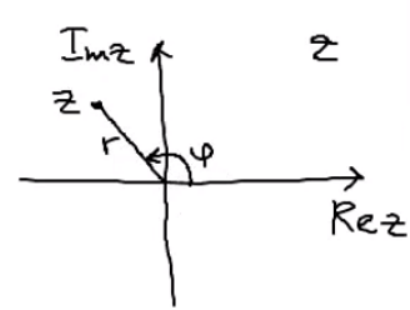
\includegraphics[scale=0.5]{img/1.png}
 
 \begin{definition*}
 Тогда \textit{модуль} числа $z$ -- $r = |z| = \sqrt{z \cdot \overline{z}} = \sqrt{x^2 + y^2}$.
  \textit{Аргумент} числа $z$ -- угол $\varphi$, такой что $x = |z| \cos \varphi,\ y = |z| \sin \varphi$. \end{definition*}
  
  На этом моменте впервые встает вопрос о многозначности  функций.
  
  \begin{definition*}
  Если мы хотим говорить про однозначно выбираемый аргумент, то пишут $\varphi = \operatorname{arg} z \in [0; 2\pi)$ или $(-\pi; \pi]$ --\textit{ главное значение} аргумента. При этом,  $\varphi = \operatorname{Arg}z =\operatorname{arg} z + 2\pi k,k \in \mathbb{Z}$ -- \textit{полный (или многозначный)}  аргумент.
  \end{definition*}

  \begin{definition*}
  \textit{Тригонометрическая запись}  комплексного числа: $z = |z| \cdot (\cos \operatorname{Arg}z + i \sin \operatorname{Arg}z)$.
  \end{definition*}

  \begin{definition*}
  \textit{Показательная форма записи}:  комплексного числа: $z = |z| \cdot e^{i\operatorname{Arg}z}$.
  \end{definition*}

  Комлпексную плоскость обычно обозначают $\mathbb{C}$.

\subsubsection{Сфера Римана и стереографическая проекция.}
На рисунке не окружность,  а сфера единичная. 

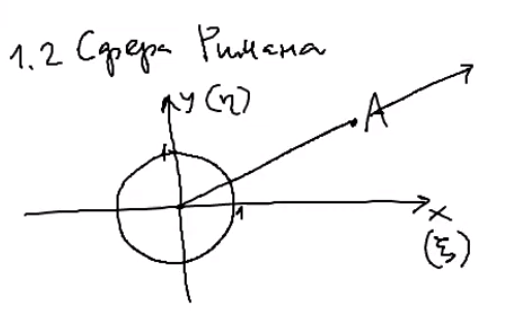
\includegraphics[scale=0.7]{img/2.png}

Рассматриваем вертикальное сечение в плоскости, содержащей ось $\zeta$ и прямую, проходящую через начало координат и точку $A$. Наша сфера выглядит следующим образом (рисунок справа):


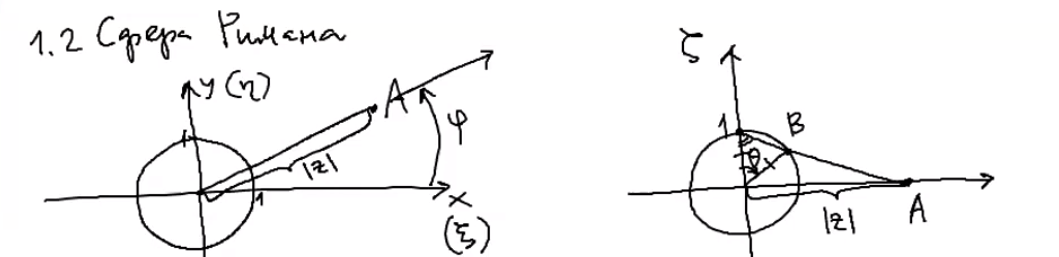
\includegraphics[scale=0.7]{img/3.png}
 
 \begin{definition*}
Отображение $B \longmapsto A$ -- \textit{стереографическая проекция.} Но для нас будет более важным обратное отображение. 
 \end{definition*}

Заметим, что $|z| = \tg \dfrac{\pi - \theta}{2} $ и $\varphi = \operatorname{arg} z$.

 Отсюда несложно вывести (по словам Маевского Е.В.), что $\xi = \dfrac{2x}{1 + |z|^2}, \eta = \dfrac{2y}{1 + |z|^2}, \zeta = \dfrac{|z|^2 - 1}{1 + |z|^2}$.  
 
 Обратные формулы: $x = \dfrac{\xi}{1 - \zeta}$ и $y = \dfrac{\eta}{1 - \zeta}$.
 \\
 \\
В действительном матанализе мы фактически имели две бесконечности (для нас было важно направление): $+\infty $ и $-\infty $. В комплексном матанализе чаще всего не имеет значения, в каком направлении мы идем в бесконечность. Поэтому рассматривается просто \textit{бесконечно удаленная точка }и обозначается $z \to \infty$. Это означает, что $|x|, |y| \to \infty$.  
\\
\\
Можно заметить, что если мы захотим добавить бесконечно удаленную точку к комплексной плоскости, то ей будет соответствовать северный полюс на сфере Римана.  Если мы добавим к комплексной плоскости бесконечно удаленную точку, то  это называется \textit{замкнутой комплексной плоскостью}: $\overline{\mathbb{C}}= \mathbb{C} \cup \{ \infty \}$.  И вот как раз замкнутую комплексную плоскость очень удобно представлять, как сферу Римана.
\\
\\
Стало непонятно, надо ли техать про  сходимость последовательности, поэтому ссылка с таймкодом на лекцию: \href{https://youtu.be/lUqrd4aP3Zc?t=1777}{тык}.
  
  
\subsubsection{Функция комплексной переменной.}
\begin{definition*}
\textit{Функция комплексной переменной }$w = f(z)$ -- отображение, заданное на одной комплексной плоскости и принимающее значения на другой комплексной плоскости. 
\end{definition*}
Считаем, что $w = u + iv$, тогда становится понятно, что $f(z) = u(z) + iv(z)$, где $u(z), v(z) $ -- вещественные функции от комплексной переменной. Еще можно представлять функцию от $z$ как функцию от двух переменных: $f(z) = \widetilde{f}(x, y)$.  Тогда $\widetilde{f}(x, y) = \widetilde{u}(x, y) + i \widetilde{v}(x, y)$.

 Замена переменной:
 \begin{align*}
 \begin{cases}
 	z = x + iy \\
 	\overline{z} = x - iy
 \end{cases} \iff 
 \begin{cases}
 x = \dfrac{z + \overline{z}}{2} \\
 y = \dfrac{z - \overline{z}}{2i}
 \end{cases} 
 \end{align*}
 Тогда $f(z) = \widetilde{f}\left(\dfrac{z + \overline{z}}{2}, \dfrac{z - \overline{z}}{2i}\right)$.
 
 \subsubsection{Определения экспоненты $e^z$ и тригонометрических функций $\sin z$, $\cos z$.}
 
 \begin{definition*}  \textit{Экспонента} $e^z$ в комплексном случае задается двумя  эквивалентными способами:
 	
 	\qquad	1) $e^z := \lim\limits_{n \to \infty} \left(1 + \dfrac zn\right)^n\ \forall z$
 	
 	\qquad	2) $e^z := \sum_{n = 0}^{\infty} \dfrac{z^n}{n!}$
 		
 	На основе этого определения доказываются все те же известные нам алгебраические свойства экспоненты для комплексного случая. 
 \end{definition*}

Тогда можем написать, что $w = e^{x + iy} = e^x \cdot e^{iy} = e^x(\cos y + i\sin y) \implies u  = e^x\cos y,\ v = e^x\sin y$.

\begin{definition*} Косинус в комплексном случае тоже задается двумя эквивалентными способами:
	
	\qquad	1) $\cos z := \dfrac{e^{iz} + e^{-iz}}{2}$ \\
	
	\qquad 2) $\cos z := \sum_{n = 0}^{\infty} \dfrac{(-1)^n z^{2n}}{(2n)!}$
	
	С помощью этих формул можно получить следующее: $$
	\cos z = \dfrac{e^{-y}(\cos x + i\sin x) + e^{y}(\cos x - i\sin x)}{2} = \cos x \ch y - i \sin x \sh y \implies  u =  \cos x \ch y, v = -\sin x \sh y $$
\end{definition*} 


\begin{definition*} Синус в комплексном случае тоже задается двумя эквивалентными способами:
	
	\qquad	1) $\sin z := \dfrac{e^{iz} - e^{-iz}}{2i}$ \\
	
	\qquad 2) $\cos z := \sum_{n = 1}^{\infty} \dfrac{(-1)^{n - 1} z^{2n - 1}}{(2n - 1)!}$
	
	С помощью этих формул можно получить следующее: $$
	\sin z =  \dfrac{e^{-y}(\cos x + i\sin x) - e^{y}(\cos x - i\sin x)}{2i} = \sin x \ch y + i \cos x \sh y \implies  u =  \sin x \ch y, v = \cos x \sh y$$
\end{definition*} 


\subsubsection{Определения многозначных функций $\sqrt[n]{z}$, $\operatorname{Ln} z$.}

\begin{definition*}
	\textit{Комплексным корнем n--ой степени } $\sqrt[n] z, \,z \neq 0$  называется каждое число $w: w^n = z$, где $ n = 2, 3, 4, \dots$
\end{definition*}


\begin{definition*}
	\textit{Полным натуральным логарифмом } $\operatorname{Ln} z$, $ \,z \neq 0$  называется каждое число $w: e^w = z$.
	Составим $z = |z| \cdot e^{i\operatorname{Arg} z} \implies \operatorname{Ln} z  = \ln |z| + i \operatorname{Arg} z = \ln |z| + i \operatorname{arg} z + i 2\pi k, k \in \mathbb{Z}$. Это пример бесконечнозначной функции.
\end{definition*}
    % Здесь НЕ НУЖНО делать begin document, включать какие-то пакеты..
% Все уже подрубается в головном файле
% Хедер обыкновенный хсе-теха, все его команды будут здесь работать
% Пожалуйста, проверяйте корректность теха перед пушем

% Здесь формулировка билета
\subsection{Докажите, что измеримые по Жордану множества образуют кольцо}

\textbf{\underline{Утв.:} } Измеримые по Жордану множества образуют кольцо\\
\textbf{\underline{Док-во:} } \\
\begin{enumerate}
    \item $\varnothing$ - пустое множество является простым, а значит измеримо.
    \item $A, B$ - измеримы, $A \cup B$ - объединение измеримых множеств измеримо. \\
Пусть $A_i \subseteq E_i$ и $\overline{\mu}(E_i\backslash A_i) < \frac{\varepsilon}{2}$, при $i = 1, 2$. \\
Тогда так как 
\[(E_1\cup E_2) \backslash (A_1\cup A_2) \subseteq (E_1\backslash A_1) \cup (E_2\backslash A_2) \]
в силу монотонности имеем 
\[\overline{\mu}((E_1\cup E_2) \backslash (A_1\cup A_2)) \leq \overline{\mu}((E_1\backslash A_1) \cup (E_2\backslash A_2)) < \frac{\varepsilon}{2} + \frac{\varepsilon}{2} = \varepsilon \]
а из этого следует, что объединение измеримо.
    \item $A, B$ - измеримы, $A \cap B $ - пересечение измеримых множеств измеримо. \\
Проведем рассуждения аналогично предыдущему пункту. \\
Так как
\[(E_1\cap E_2) \backslash (A_1\cap A_2) \subseteq (E_1\backslash A_1) \cup (E_2\backslash A_2) \]
в силу монотонности имеем
\[ \overline{\mu}((E_1\cap E_2) \backslash (A_1\cap A_2)) \leq \overline{\mu}((E_1\backslash A_1) \cup (E_2\backslash A_2)) < \frac{\varepsilon}{2} + \frac{\varepsilon}{2} = \varepsilon \]
а из этого следует, что пересечение измеримо.
    \item $A, B$ - измеримы, $ A \backslash B$ - разность измеримых множеств измерима. \\
Пусть $A_i \subseteq E_i$, при $i = 1, 2$ и простые множества $E_i$ таковы, что $\overline{\mu}(E_1\backslash A_1) < \frac{\varepsilon}{2}$, а $E_2 \backslash A_2 \subseteq E_2'$, где $\mu(E_2') < \frac{\varepsilon}{2}$. \\
Обозначим
\[A = A_1 \backslash A_2, \text{ и } E = (E_1\backslash E_2) \cup E_2'\]
Докажем, что $A\subseteq E$. Из всех возможных вариантов рассмотрим следующий. Пусть $x \in A_1$ и $x \not\in A_2$. Тогда $x \in E_1$, а если $x\in E_2$, то $x \in E_2'$. Все прочие случаи тривиальны. \\
Теперь докажем, что
\[(E\backslash A) \subseteq (E_1\backslash A_1) \cup E_2'\]
Снова из всех возможных вариантов рассмотрим следующее. Пусть $x \in E$ и $x \not\in A $. Отсюда пусть $x \in E_1$ и $x \not\in E_2$. Если $x \in A_1$, то либо $x \in A$, что противоречит первоначальному условию, либо $x \in A_1 \cap A_2$, что также невозможно, так как $x \not\in E_2$. Отсюда следует, что $x \not\in A_1$. Все прочие случаи тривиальны. \\
Далее имеем
\[\overline{\mu}(E\backslash A) \leq \overline{\mu}(E_1\backslash A_1) + \overline{\mu}(E_2') = \varepsilon\]
Из чего следует, что разность измеримых множеств измерима.
\end{enumerate}
Все необходимые условия выполнены а это значит, что измеримые множества образуют кольцо. 
\begin{flushright}
$\blacksquare$
\end{flushright}



    \newcommand{\darrowwtextover}[3]{%
\raisebox{0pt}[0pt][0pt]{%
$\overset{\mathclap{\substack{#1\\\left\downarrow\vcenter{\hrule height #2}\right.}}}{#3}%
$}%
}

\subsection{Тригонометрический ряд Фурье.
Теорема о сходимости тригонометрического ряда Фурье в средне-квадратичном (без доказательства полноты тригонометрической системы).
Представление частичной суммы ряда Фурье через ядро Дирихле.
Лемма Римана.
Условие Дини и теорема о поточечной сходимости ряда Фурье.
Разложение $\sin$ в бесконечное произведение.}

Лекции 3.8 (примерно с часа) и 3.9

\subsubsection{Тригонометрический ряд Фурье}

Тригонометрическая система: $\left\{ 1, \cos x, \sin x, \cos 2x, \dotsc \right\}$.
Ряд Фурье, который пользуется именно этой системой, и является тригонометрическим.

\subsubsection{Теорема о сходимости тригонометрического ряда Фурье в средне-квадратичном
(без доказательства полноты тригонометрической системы).}

Если тригонометрическая система $\left\{ 1, \cos x, \sin x, \cos 2x, \dotsc \right\}$ полна
в $\mathcal{R}_2 \left( [-\pi, \pi], \RR \right)$
(а это так, но без доказательства), то:
\begin{enumerate}
\item
$\forall f \in \mathcal{R}_2$ ряд Фурье сходится в $\mathcal{R}_2$ к $f$.
(Это не поточечная сходимость, а среднеквадратичная!)
\[
    f(x) \underset{\mathcal{R}_2}{=} \frac{a_0}{2} +
    \sum_{n=1}^{\infty} \left( a_n \cos nx + b_n \sin nx \right)
\]
\item
Выполняется равенство Парсеваля
\[
    \frac{1}{\pi} \int_{-\pi}^{\pi} f^2(x) dx = \frac{a_0^2}{2} +
    \sum_{n=1}^{\infty} \left( a_n^2 + b_n^2 \right)
\]
\end{enumerate}

Если функция не в $\mathcal{R}_2 \left( [-\pi, \pi], \RR \right)$, а в
$\mathcal{R}_2 \left( [-\pi, \pi], \CC \right)$, то
\[
    f(x) \underset{\mathcal{R}_2}{=} \sum_{n=-\infty}^{\infty} c_n e^{inx},
    \text{ где } c_n = \frac{1}{2\pi} \int_{-\pi}^{\pi} f(x) e^{-inx} dx
\]
, а равенство Парсеваля выглядит как
\[
    \frac{1}{2\pi} \int_{-\pi}^{\pi} |f(x)|^2 dx =
    \sum_{n=-\infty}^{\infty} |c_n|^2
\]

\subsubsection{Представление частичной суммы ряда Фурье через ядро Дирихле.}
$f: [-\pi, \pi] \rightarrow \RR$ — продолжаем периодически на всю вещественную прямую,
разрывы нам здесь не страшны
\begin{flalign*}
    & \text{Частичная сумма Фурье} \quad S_n(x) =
    \frac{a_0}{2} + \sum_{k=1}^n \left( a_k \cos kx + b_k \sin kx \right) =
    \sum_{k=-n}^n c_k e^{ikx} = \\
    & = \sum_{k=-n}^n \left( \frac{1}{2\pi} \int_{-\pi}^{\pi} f(t) e^{-ikt} dx \right) e^{ikx} =
    \text{\em суммирование конечное, поэтому заносим под интеграл} = \\
    & = \frac{1}{2\pi} \int_{-\pi}^{\pi} f(t) D_n(x - t) dt = \textcolor{blue}{(*)}\\
    & \left. \begin{array} {lr}
    D_n(u) = \sum_{k=-n}^n e^{ikn} = \frac{e^{i(n+1)u} - e^{-inu}}{e^{iu} - 1}
    \left( \frac{\phantom{w}\frac{1}{e^{in/2}}\phantom{w}}{\frac{1}{e^{in/2}}} \right) =
    \frac{\sin \left( n + \frac{1}{2} \right)u}{\sin \frac{1}{2} u}, & u \neq 2 \pi k \\
    D_n(u) = 2n + 1, & u = 2 \pi k
    \end{array} \right\}
    \parbox{10em}{\raggedright — Ядро Дирихле.\\
              Доопределили там, где потребовалось} \\
    & \text{Свойства:} \qquad
    D_n(u)\; 2 \pi \text{ периодическая}; \quad
    D_n(u) = _n(-u); \quad
    \frac{1}{2\pi} \int_{-\pi}^{\pi} D_n(u) du = 1 \\
    & \text{Заметим, что если } g(t) \text{ — } T \text{ периодическая, то }
    \int_0^T g(t) dt = \int_x^{T+x} g(t) dt \\
    & \textcolor{blue}{(*)} = \frac{1}{2\pi} \int_{-\pi}^{\pi} f(t) D_n(x - t) dt = \left\{ t' = x - t \right\}
    \frac{1}{2\pi} \int_{x-\pi}^{x + \pi} f(x - t') D_n(t') dt' =
    \frac{1}{2\pi} \int_{-\pi}^{\pi} f(x - t') D_n(t') dt' = \\
    & = \frac{1}{2\pi} \int_{-\pi}^{0} f(x - t') D_n(t') dt' +
    \frac{1}{2\pi} \int_{0}^{\pi} f(x - t') D_n(t') dt' = \left\{ \begin{array} {c}
        t^* = -t' \\
        \text{слева}
    \end{array}  \right\} = \\
    & = \frac{1}{2\pi} \int_{0}^{\pi} f(x + t^*) D_n(t^*) dt^* +
    \frac{1}{2\pi} \int_{0}^{\pi} f(x - t') D_n(t') dt' = \text{переобозначим } t =
    \frac{1}{2\pi} \int_0^{\pi} D_n(t) \left( f(x + t) + f(x - t) \right) dt
\end{flalign*}

\subsubsection{Лемма Римана.}
\begin{lemma*}
Если $f(\omega_1, \omega_2) \rightarrow \RR$ (бесконечности тоже можно) локально интегрируема
(интегрируема на любом подотрезке) и абсолютно интегрируема хотя бы в несобственном смысле на всем
$(\omega_1, \omega_2)$, то
\[
    \int_{\omega_1}^{\omega_2} f(x) e^{i \lambda x} dx \xrightarrow[\lambda \to \infty]{} 0
\]
\end{lemma*}
\begin{proof}
Так как $f$ абсолютно интегрируема, $\exists [a, b] \subset (\omega_1, \omega_2):
\left| \int_{\omega_1}^{\omega_2} f(x) e^{i \lambda x} dx - \int_a^b f(x) e^{i\lambda x}dx \right| \leq \eps$.
Утверждать так можем потому что $|f(x) e^{i\lambda x} | = |f(x)| \Rightarrow f(x)e^{i \lambda x}$ тоже абс. инт.

Рассмотрим нижнюю сумму Дарбу:
$0 \leq \int_a^b f(x) dx - \sum_{j=1}^n m_j \Delta x_j < \eps$. Здесь возникает разбиение
$a = x_0 < x_1 < x_2 < \dotsb < x_n = b$. Построим по нему кусочную функцию
\[
    h(x) = \left\{ \begin{array} {lr}
        m_1, & x \in [x_0, x_1) \\
        m_2, & x \in [x_1, x_2) \\
        \hdotsfor{2} \\
        m_n, & x \in [x_{n-1}, x_n]
    \end{array} \right.
\]
Заметим тогда, что
\begin{flalign*}
    & 0 \leq
    \left| \int_a^b f(x) e^{i \lambda x} dx - \int_a^b h(x) e^{i\lambda x} dx \right| \leq
    \int_a^b |f(x) - h(x)| \underbrace{|e^{i \lambda x}|}_{= 1} dx =
    \underbrace{\int_a^b |f(x) - h(x)| dx}_{\text{Дарбу!}} < \eps
\end{flalign*}

Разложим $h(x)$ по частям
\begin{flalign*}
    & \int_a^b h(x) e^{i \lambda x} dx = \sum_{j=1}^n \int_{x_{j-1}}^{x_j} m_j e^{i \lambda x} dx
    \darrowwtextover{\text{руками взять интеграл}}{1em}{=}
    \frac{1}{i\lambda} \sum_{j=1}^n m_j \left( e^{i\lambda x_j} - e^{i\lambda x_{j-1}} \right)
    \xrightarrow[\lambda \to \infty]{} 0
\end{flalign*}
Так как все множители под суммой ограничены, $n$ от лямбды не зависит, а мы еще делим на бесконечно большую лямбду

А теперь вспоминаем те интегралы, которые отличаются друг от друга на сколь угодно малую величину:
\begin{flalign*}
    & \int_a^b h(x) e^{i\lambda x} dx \to 0 \;\; \implies \;\; \int_a^b f(x) e^{i \lambda x} dx \to 0
    \;\; \implies \;\; \int_{\omega_1}^{\omega_2} f(x) e^{i \lambda x} dx \to 0
\end{flalign*}

\end{proof}

На самом деле функция может быть и комплекснозначной, для этого придется раскрыть $e^{i\lambda x}$
на синус и косинус и силой рук посчитать. Получается и вещественная часть $f(x) e^{i\lambda x}$
будет интегрироваться в ноль, и комплексная.
Доказательства этого не требуется, но стоит запомнить для следующего пункта.

\subsubsection{Условие Дини и теорема о поточечной сходимости ряда Фурье.}
\textbf{Запомните ПМИшники, }
$\sum_{n = -N}^N c_n e^{inx} = \frac{a_0}{2} + \sum_{n=1}^{N} \left( a_n \cos nx + b_n \sin nx \right)$

\begin{theorem*}
Пусть $f: \RR \to \CC$ $2 \pi$ периодическая (хотя можно и другой период, но мы упрощаем себе жизнь),
абсолютно интегрируемая на $[-\pi, \pi]$ и удовлетворяет в точке $x_0$ условию Дини:
\begin{enumerate}
\item $\exists f(x_0 \pm 0) $ — конечные
\item $\exists \eps > 0: \quad
    \int_0^{\eps} \left( \frac{f(x_0 - t) - f(x_0 - 0)}{t} + \frac{f(x_0 + t) - f(x_0 + 0)}{t} \right) dt$
    — сходится абсолютно
\end{enumerate}

Тогда разложение Фурье функции $f$ сходится в точке $x_0$:
$\sum_{n=-N}^{N} c_n e^{inx_0} \to \frac{f(x_0 - 0) + f(x_0 + 0)}{2} $

\end{theorem*}

\begin{proof}
Тут несложно, но много писать

\begin{flalign*}
    & S_N(x_0) - \frac{f(x_0 - 0) + f(x_0 + 0)}{2} = \\
    & = \frac{1}{2 \pi} \int_0^{\pi} \left( f(x_0 - t) + f(x_0 + t) \right)
    \frac{\sin \left( N + \frac{1}{2} \right) t}{\sin \frac{t}{2}} dt -
    \frac{f(x_0 - 0) + f(x_0 + 0)}{2} \cdot
    \darrowwtextover{\scalebox{0.75}{$\displaystyle
        \frac{2}{2\pi} \int_{0}^{\pi} \frac{\sin \left( N + \frac{1}{2} \right) t}{\sin \frac{t}{2}} dt
    $}}{1em}{
        \underbrace{\frac{1}{2\pi} \int_{-\pi}^{\pi} \frac{\sin \left( N + \frac{1}{2} \right) t}{\sin \frac{t}{2}} dt}_{=1}
    } = \\
    & = \frac{1}{2 \pi} \int_0^\pi
    \Big( \left( f(x_0 - t) + f(x_0 + t) \right) - \left( f(x_0 - 0) + f(x_0 + 0) \right) \Big)
    \frac{\sin \left( N + \frac{1}{2} \right) t}{\sin \frac{t}{2} } dt = \\
    & = \frac{1}{\pi} \int_0^\pi
    \underbracket{
        \left( \frac{f(x_0 - t) - f(x_0 - 0)}{t} + \frac{f(x_0 + t) - f(x_0 + 0)}{t} \right)
    }_{\text{абс. инт. по условию Дини}}
    \underbrace{\frac{t}{2 \sin\frac{t}{2} }}_{\mathclap{1 \text{ при } t \to 0}}
    \underbracket{\sin \left( N + \frac{1}{2} \right) t}_{\mathclap{\sim \Im e^{i \lambda t}}} dt
    \xrightarrow[N \to \infty]{} 0 \text{ по Риману}
\end{flalign*}
Здесь в последнем переходе как раз было махание руками про комплексные значения,
объясняется что ``если очень захотеть, то можно и доказать, но долго и неинтересно''
\end{proof}


\begin{definition*} 
Функция $f: [a, b] \to \CC$ называется кусочно-дифференцируемой, если 
\begin{enumerate} 
\item множество точек разрыва $M$ конечно, и каждая точка разрыва первого рода 
    (слева справа разные конечные значения)
\item Функция дифференцируема во всех точках $x \in [a, b] \setminus M$
\item $\forall x_0 \in M$ существуют конечные левая и правая производные.
\end{enumerate} 
\end{definition*} 

Кусочно-дифференцируемая функция удовлетворяет условию Дини, чем сейчас и воспользуемся


\subsubsection{Разложение $\sin$ в бесконечное произведение.}

Рассмотрим функцию $f(x) = \cos ax, [-\pi, \pi], |a| < 1$. Периодически продолжим на всю вещественную прямую, 
получится кусочно-дифференцируемая функция. А это значит, что с полученным рядом Фурье будет равенство.

Функция четная, поэтому $b_n = 0$.
\begin{flalign*}
    & a_n = \frac{1}{\pi} \int_{-\pi}^{\pi} \cos ax \cos nx dx = 
    \frac{(-1)^n \sin \pi a}{\pi} \frac{2a}{a^2 - n^2} \\
    & \cos ax = \frac{2a \sin \pi a}{\pi} \left( \frac{1}{2a^2} + 
    \sum_{n=1}^{\infty} \frac{(-1)^n}{a^2 - n^2} \cos nx  \right) \text{ верно } \forall x \in [-\pi, \pi] \\
    & \pmb{x = \pi\colon} \ctg \pi a - \frac{1}{\pi a} = \frac{2a}{\pi} \sum_{n=1}^{\infty} \frac{1}{a^2 - n^2}
    \text{ сходится равномерно при } a \in [-a_0, a_0]; a_0 < 1
    \text{ — проинтегрируем! (в $a = 0$ доопр.)} \\
    & \int_0^x \left( ctg \pi a - \frac{1}{\pi a} \right) da = 
    \frac{1}{\pi} \sum_{n=1}^{\infty} \int_0^x \frac{2a}{a^2 - n^2} da \quad \text{ интегрируем обе стороны} \\
    & \ln \frac{\sin \pi x}{\pi x} = \sum_{n=1}^{\infty} \ln(1 - \frac{x^2}{n^2}), \quad |x| < 1 \\
    & \frac{\sin \pi x}{\pi x} = \prod_{n=1}^{\infty} \left( 1 - \frac{x^2}{n^2} \right) \text{ ну вот и все}
\end{flalign*}

    \subsection{Тригонометрический ряд Фурье. Теорема о почленном дифференцировании ряда Фурье. Теорема о связи гладкости функции и скорости убывания ее коэффициентов Фурье. Теорема о связи гладкости функции и скорости сходимости ее ряда Фурье. Теорема о полноте тригонометрической системы.}

\subsubsection{Теорема о почленном дифференцировании ряда Фурье.}
\begin{theorem*} Если непрерывная функция $f \in C(\left[ -\pi; \pi \right], \mathbb{C})$, принимающая на концах отрезка $\left[ -\pi; \pi \right]$ равные значения, т.е. $f(\pi) = f(-\pi)$, кусочно непрерывно дифференцируема на $\left[ -\pi; \pi \right]$, то ряд Фурье ее производной $f' \sim \sum_{-\infty}^{\infty} c_n(f') \cdot e^{inx}$ может быть получен формальным дифференцированием ряда Фурье самой функции $f \sim \sum_{-\infty}^{\infty} c_n(f) \cdot e^{inx}$, то есть получаем  $c_n(f') = inc_n(f),\, n \in \mathbb{Z}$.
\end{theorem*}
\begin{proof} Из определения коэффициентов Фурье (\ref{subsubsec:label1}) интегрированием по частям находим \begin{align*}
		c_n(f') = \dfrac{1}{2\pi}\int_{-\pi}^{\pi} f'(x)e^{-inx}\, dx = \dfrac{1}{2\pi} f(x)e^{-inx}\biggl|_{-\pi}^{\pi} + \dfrac{in}{2\pi}\int_{-\pi}^{\pi} f(x)e^{-inx}\, dx = inc_n(f) \text{, т.к. } f(\pi)e^{-in\pi} - f(-\pi)e^{in\pi} = 0.
	\end{align*}
\end{proof}

\subsubsection{Теорема о связи гладкости функции и скорости убывания ее коэффициентов Фурье.}
\begin{theorem*} Пусть $f(x): \left[-\pi; \pi\right] \to \mathbb{C}$ такова, что
	\begin{itemize}
		\item[1)] функция $(m-1)$ раз непрерывно дифференцируема на $\left[ -\pi; \pi \right]$, $m \in \mathbb{N}$,
		\item[2)] $f^{(k)}(-\pi) = f^{(k)}(\pi)$ при всех $k = 0,1, \dotsc, (m-1)$,
		\item[3)] функция $(m)$ раз кусочно--непрерывно дифференцируема (другими словами: $f(x)\text{ имеет на } \left[ -\pi; \pi \right]$ кусочно непрерывную производную $f^{(m)}$ порядка $m$),
	\end{itemize}
	тогда $c_n(f^{(m)}) = (in)^m \cdot c_n(f),\, n \in \mathbb{Z}$ и $\left|c_n(f)\right| = \dfrac{\gamma_n}{|n|^m} = o\left(\dfrac{1}{n^m}\right)$ , причем $\gamma_n = |c_n(f^{(m)})|$ и ряд $\sum_{-\infty}^{\infty} \gamma_n^2$ сходится при  $n \to \infty, n \in \mathbb{Z}$.
\end{theorem*}
\begin{proof} Первое соотношение получается в результате $m$--кратного использования равенства $c_n(f') = inc_n(f)$ (из пункта выше): $c_n(f^{(m)}) = (in) \cdot c_n(f^{(m-1)}) = \dotsc  = (in)^mc_n(f)$. 
	
	Второе соотношение получается с учетом неравенства Бесселя (\ref{subsubsec:label2}): $\sum_{-\infty}^{\infty} |c_n(f^{(m)})|^2 \leqslant \dfrac{1}{2\pi} \int_{-\pi}^{\pi}|f^{(m)}|^2(x)\, dx$ -- это число $\implies \gamma_n = |c_n(f^{(m)})| \to 0$, и ряд $\sum_{-\infty}^{\infty} |c_n(f^{(m)})|^2 = \sum_{-\infty}^{\infty} \gamma_n^2 $ сходится.  Следовательно,  $c_n(f) = o\left(\dfrac{1}{n^m}\right)$.
	
\end{proof}
\subsubsection{Теорема о связи гладкости функции и скорости сходимости ее ряда Фурье.}
\begin{theorem*} Если $f(x): \left[-\pi; \pi\right] \to \mathbb{C}$ такова, что
	\begin{itemize}
		\item[1)] функция $(m-1)$ раз непрерывно дифференцируема на $\left[ -\pi; \pi \right]$, $m \in \mathbb{N}$,
		\item[2)] $f^{(k)}(-\pi) = f^{(k)}(\pi)$ при всех $k = 0,1, \dotsc, (m-1)$,
		\item[3)] функция $(m)$ раз кусочно--непрерывно дифференцируема (другими словами: $f(x)\text{ имеет на } \left[ -\pi; \pi \right]$ кусочно непрерывную производную $f^{(m)}$ порядка $m \geqslant 1$),
	\end{itemize}
	то ряд Фурье функции $f$ сходится к $f$ абсолютно и равномерно на отрезке $\left[-\pi; \pi\right]$, причем отклонение $n$--й частичной суммы $S_n(x)$ ряда Фурье от $f(x)$ на всем отрезке $\left[-\pi; \pi\right]$ имеет оценку $|f(x) - S_n(x)| \leqslant \dfrac{\varepsilon_n}{n^{m - 1/2}}$, где ${\varepsilon_n}$ -- стремящаяся к нулю последовательность положительных чисел при $n \to \infty$.
\end{theorem*} 
\begin{proof} Частичную сумму ряда Фурье(\ref{subsubsec:label3}) запишем в компактной форме: $S_n(x) = \sum_{-n}^{n} c_k(f)e^{ikx}$.
	
	В соответствии с условиями на функцию $f$ и по теореме о связи гладкости функции и скорости убывания ее коэффициентов Фурье имеем:
	$\left|c_k(f)\right| = \dfrac{\gamma_k}{|k|^m}$, причем $\sum \dfrac{\gamma_k}{|k|^m} < \infty$ (поскольку $0 \leqslant \dfrac{\gamma_k}{|k|^m} \leqslant \dfrac12 \left(\gamma_k^2 + \dfrac{1}{k^{2m}}\right)$ по неравенству о среднем и  $m \geqslant 1$, имеем $\sum \dfrac{\gamma_k}{|k|^m} < \infty$). Значит, последовательность $S_n(x)$ на  отрезке $\left[ -\pi; \pi \right]$ равномерно сходится по мажорантному признаку Вейерштрасса для рядов (или критерию Коши для последовательностей).
	
	В силу достаточного условия сходимости ряда Фурье в точке предел $S(x)$ последовательности $S_n(x)$ совпадает с $f(x)$, поскольку функция $f$ удовлетворяет условиям Дини в каждой точке отрезка $\left[ -\pi; \pi \right]$ и т.к.  	$f(-\pi) = f(\pi)$	, то функция $f$ периодически продолжается на $\mathbb{R}$ с сохранением условий Дини в любой точке $x \in \mathbb{R}$.
	
	Переходим к оценке. Используем последнее равенство из конца формулировки теоремы 11.2:
	\begin{align*}
		|f(x) - S_n(x)| = |S(x) - S_n(x)| = \left|\sum_{\pm k = n + 1}^{\infty} c_k(f)e^{ikx} \right| &\leqslant \sum_{\pm k = n + 1}^{\infty} |c_k(f)| =  \sum_{\pm k = n + 1}^{\infty} \dfrac{\gamma_k}{|k|^m} \leqslant \\
		&\leqslant \left( \sum_{\pm k = n + 1}^{\infty} \gamma_k^2\right)^{1/2} \left( \sum_{\pm k = n + 1}^{\infty} 1/k^{2m}\right)^{1/2}
	\end{align*}	
	Первый множитель в правой части неравенства Коши--Буняковского стремится к нулю при $n \to \infty$, т.к. $\sum_{-\infty}^{\infty} \gamma_k^2 < \infty$. 
	
	Далее (см. рис.104) оценка:
	\begin{align*}
		\sum_{k = n + 1}^{\infty} \dfrac{1}{k^{2m}} \leqslant \int_{n}^{\infty} \dfrac{dx}{x^{2m}} = \dfrac{1}{2m-1} \cdot \dfrac{1}{n^{2m-1}}.
	\end{align*}
	\begin{center}
		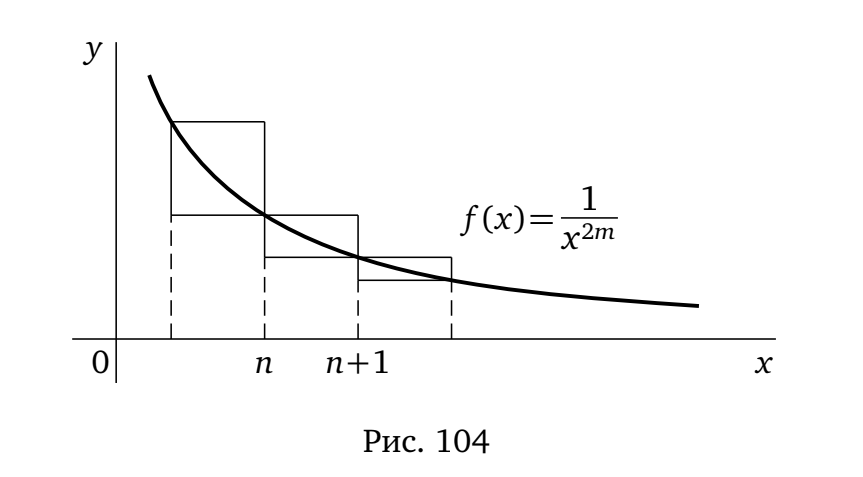
\includegraphics[scale=0.5]{img/pic104.png}
	\end{center}
	Таким образом, получается то, что и утверждает теорема.
\end{proof}

\subsubsection{Теорема о полноте тригонометрической системы.}

\begin{theorem*} \ Любая функция $f \in \mathcal{R}_2(\left[ -\pi; \pi \right], \mathbb{R})$ (т.е. $f$ интегрируема на любом отрезке $\left[a; b\right] \subset \left( -\pi; \pi \right)$ и $f^2(x)$ интегрируема хотя бы в несобственном смысле на отрезке $\left[ -\pi; \pi \right]$) может быть сколь угодно точно приближена (по--научному: апроксимирована) в средне--квадратичном тригонометрическими многочленами.
\end{theorem*}
\begin{proof} Любую функцию $f \in \mathcal{R}_2$  можно сколь угодно точно  приблизить финитной функцией $g \in \mathcal{R}_2$ на $\left[-\pi; \pi\right]$, интегрируемой по Риману на этом отрезке (функция $g$ называется \textit{финитной} на $[-\pi; \pi]$, если существует $[a; b]\subset(-\pi; \pi)$ и $g = 0$ при $x \in [-\pi; \pi] \backslash [a; b]$). Функцию $g$ мы приближаем кусочно постоянной функцией $h$ на отрезке $[-\pi; \pi]$.   Функцию $h$ приближаем ломанной функцией $l$, которая на концах отрезка будет равна нулю. Тогда ломанная $l$ -- это кусочно непрерывная дифференцируема функция, и она сколь угодно точно приближается тригонометрическим многочленом.  Из всего этого получаем, что любая функция $f \in \mathcal{R}_2$  по норме пространства $\mathcal{R}_2$  сколь угодно точно приближается  тригонометрическим многочленом.
\end{proof}
    % Здесь НЕ НУЖНО делать begin document, включать какие-то пакеты..
% Все уже подрубается в головном файле
% Хедер обыкновенный хсе-теха, все его команды будут здесь работать
% Пожалуйста, проверяйте корректность теха перед пушем

% Здесь формулировка билета
\subsection{Докажите, что произведение разбиений является измельчением и одного, и другого разбиения} 

\textbf{\underline{Утв.:} } Пусть $\tau$ и $\tau'$ - произвольные разбиения некоторого множества, тогда $\tau \cdot \tau'$ является измельчением $\tau$ и $\tau'$\\
\textbf{\underline{Док-во:} } Пусть $D_i \subseteq \tau$ и $D_i' \subseteq \tau'$, тогда так как 
\[\forall i \in \{1, ..., n\} \ D_i = D_i \cap D = D_i \cap (\bigsqcup\limits_jD_j) = \bigsqcup\limits_j(D_i\cap D_j')\]
По определению произведения $D_i \cap D_j' \subseteq \tau\cdot\tau'$, а значит по определению измельчения $\tau\cdot\tau'$ является измельчением  $\tau$ \\
($\tau'$ также является измельчением; доказывается симметрично)
\begin{flushright}
$\blacksquare$
\end{flushright}


    \subsection{Однозначные особые точки: устранимая особенность, полюс, существенная особенность. Голоморфность функции, доопределенной по непрерывности в устранимой особой точке. Порядок полюса функции $f(z)$ и порядок нуля функции $\frac{1}{f(z)}$. Теорема Сохоцкого о существенно особой точке.}


\subsubsection{Однозначные особые точки: устранимая особенность, полюс, существенная особенность.}
\begin{definition*}
Точка $z_0$ называется изолированной особой точкой однозначного характера функции $f$, если
$\\\exists\delta:$ $f$ голоморфна в проколотой окрестности $0<|z-z_0|<\delta$, но не является голоморфной ни в каком круге $|z-z_0|<r$
\end{definition*}
Классификация:
\begin{itemize}
    \item $\exists\lim\limits_{z\rightarrow z_0} f(z)\in\mathbb{C}\iff$ устранимая особенность
    \item $\exists\lim\limits_{z\rightarrow z_0} f(z)=\infty\iff$полюс
    \item $\not\exists\lim\limits_{z\rightarrow z_0}f(z)\iff$ существенная особенность
\end{itemize}


\subsubsection{Голоморфность функции, доопределенной по непрерывности в устранимой особой точке.}
\begin{theorem*}
Если $z_0~-~$устранимая особенность функции $f$ и $\lim\limits_{z\rightarrow z_0} f(z)=a\in\mathbb{C}$, то $\tilde{f}(z)=\begin{cases}
f(z),&\ z\ne z_0\\
a,&\ z=z_0.
\end{cases}$

\text{голоморфна в окрестности точки} $z_0$
\end{theorem*}
\begin{proof}
Пусть $f$ голоморфна в $0<|z-z_0|<\delta$, $\varepsilon_1<\varepsilon<\delta$  и $\varepsilon_1<|z-z_0|<\varepsilon$
Тогда по формуле Коши, получаем, что 
$$
f(z)=\dfrac{1}{2\pi i}\oint\limits_{\partial D}\dfrac{f(\zeta)}{\zeta-z}d\zeta\underbrace{=}_{\textcolor{red}{(*_1)}} \dfrac{1}{2\pi i}\oint\limits_{|\zeta-z_0|=\varepsilon}\dfrac{f(\zeta)}{\zeta-z}d\zeta-\dfrac{1}{2\pi i}\oint\limits_{|\zeta-z_0|=\varepsilon_1}\dfrac{f(\zeta)}{\zeta-z}d\zeta\underbrace{=}_{\textcolor{red}{(*_2)}}\dfrac{1}{2\pi i}\oint\limits_{|\zeta-z_0|=\varepsilon}\dfrac{f(\zeta)}{\zeta-z}d\zeta\  \ \begin{bmatrix} \text{при}\ \varepsilon_1\rightarrow 0 \\ z\ne z_0 \end{bmatrix}
$$

Объяснения:
   $\\\textcolor{red}{(*_1)}$: Граница множества $D$ состоит из двух окружностей: внешней (радиуса $\varepsilon$,  которая обходится в положительном направлении (против часовой стрелки) и внутренней (радиуса $\varepsilon_1$), которая обходится в отрицательном направлении (по часовой стрелке). Заодно сразу поменяем знак перед интегралом по внутренней окружности, для того, чтобы написать его в положительном направлении.

   $\textcolor{red}{(*_2)}$: Оценим сверху модуль второго интеграла:
   $$
   \underbrace{\left|\dfrac{1}{2\pi i}\oint \limits_{|\zeta-z_0|=\varepsilon_1}\dfrac{f(\zeta)}{\zeta-z}d\zeta\right|}_{\text{интеграл второго рода}}\leq\dfrac{1}{2\pi i}\underbrace{\oint\limits_{|\zeta-z_0|=\varepsilon_1}\left|\dfrac{f(\zeta)}{\zeta-z}\right|dl}_{\text{интеграл первого рода}}
   $$
   Затем оценим саму подынтегральную функцию:
   $$
   \left.
     \begin{array}{ccc}
       f(\zeta)=a+o(1)\ \text{при}\ \varepsilon_1\rightarrow 0 \\
       |\zeta-z|\geq|\underbrace{t-z_0}_{\text{число}}|-\varepsilon_1 \\
       \oint\limits_{|\zeta-z_0|=\varepsilon_1} dl=2\pi\varepsilon_1
     \end{array}
   \right\}\Rightarrow \dfrac{1}{2\pi i}\underbrace{\oint\limits_{|\zeta-z_0|=\varepsilon_1}\left|\dfrac{f(\zeta)}{\zeta-z}\right|dl}_{\text{интеграл первого рода}}\xrightarrow[\varepsilon_1\rightarrow 0]{}0
   $$
Вернемся к получившемуся выражению для функции $f(z)$

Так как мы перешли к пределу, мы можем сказать, что во всех точка $z$, включая $z_0$, можно понимать левую часть выражения как $\tilde{f}(z)$, тогда получим:
$$
\widetilde{f}(z)=\dfrac{1}{2\pi i}\oint\limits_{|\zeta-z_0|=\varepsilon}\dfrac{f(\zeta)}{\zeta-z}d\zeta\  \ \begin{bmatrix} \text{при}\ \varepsilon_1\rightarrow 0 \\ |z- z_0|<\delta \end{bmatrix}
$$
Если мы применим к данному интегралу рассуждения, которые мы применяли при доказательстве аналитичности голоморфной функции (11 билет), получим, что функция представленная данным образом аналитична в точке $z_0$, а отсюда следует, что она голоморфна в точке $z_0$.
Ну и напоследок, если мы в этот интеграл вместо $z$ подставим $z_0$, в силу произвольности $\varepsilon$, устремив $\varepsilon$ к нулю, мы получим, что $\widetilde{f}(z_0)=a$.
\end{proof}


\subsubsection{Порядок полюса функции $f(z)$ и порядок нуля функции $\frac{1}{f(z)}$.}
\begin{definition*}
Полюс это точка, такая что в проколотой окрестности этой точки функция голоморфна, а в самой этой точке в пределе получается бесконечное значение.
\end{definition*}

Пускай $f(z)\xrightarrow[z\rightarrow z_0]{}\infty$, то есть $z_0~-~$ полюс

Рассмотрим функцию $g(z)=\dfrac{1}{f(z)}$, тогда $g(z)\xrightarrow[z\rightarrow z_0]{}0$ и $g(z)$ будет голоморфной в проколотой окрестности точки $z_0$ (так как $f(z)$ голоморфна в проколотой окрестности точки $z_0$ и не обращается в 0), отсюда делаем вывод, что $g(z)$ имеет устранимую особенность.

Доопределим функцию $g(z)$ в точке $z_0$, получим новую функцию $\widetilde{g}(z)=\begin{cases}
\dfrac{1}{f(z)},\ z\ne z_0,\\
0,\ z= z_0.
\end{cases}$ которая будет голоморфной в точке $z_0$, а значит будет аналитической, мы можем представить ее в виде степенного ряда:
$$
\widetilde{g}(z)=\sum\limits_{k=0}^\infty c_{k}(z-z_0)^k\text{ так как}\ \widetilde{g}(z_0)=0 \text{ то}\ c_0=..=c_n=0, c_{n+1}\ne 0\Rightarrow\\ \widetilde{g}(z)=(z-z_0)^n(\underbrace{c_{n+1}+c_{n+2}(z-z_0)+..)}_{h(z)}
$$
\begin{definition*}
В такой ситуации говорят, что $\widetilde{g}(z)$ имеет нуль $n-$ого порядка.
\end{definition*}

Распишем тогда как будет выглядеть изначальная функция $f(z)$:
$$
f(z)=\dfrac{1}{g(z)}=\dfrac{1}{(z-z_0)^n}\cdot \underbrace{\dfrac{1}{h(z)}}_{\text{голоморфна в}\ z_0}
$$
\begin{definition*} Число $n$ в полученном выражении называется называется порядком полюса. Функция $f(z)$ имеет полюс $n-$ого порядка.
\end{definition*}
\subsubsection{Теорема Сохоцкого о существенно особой точке.}
\begin{theorem*}
Если $z_0~-~$существенно особая точка функции $f$, то
$$
\forall a\in\overline{\mathbb{C}}\  \exists\{z_n\}\colon z_n\rightarrow z_0,\ f(z_n)\rightarrow a
$$
\end{theorem*}
\begin{proof}
$\\$
\begin{itemize}
    \item $a=\infty$ Если функция ограничена в $0<|z-z_0|<\delta$ то $z_0~-~$ устранимая особенность, но так как мы знаем, что $z_0$ не является устранимой особенностью, то функция $f$ не ограничена в кольце  $0<|z-z_0|<\delta$, а значит $\exists\{z_n\}:\ z_n\rightarrow z_0,\ f(z_n)\rightarrow \infty$
    \item Если $\forall\delta\ \exists z:\ 0<|z-z_0|<\delta\ f(z)=a$, тогда $\exists\{z_n\}:\ 0<|z_n- z_0|<\dfrac{1}{n}\ f(z_n)=a$ (выбрали последовательность, на которой функция в точности принимает значение $a$)
    \item $\exists\delta:\ 0<|z-z_0|<\delta\ f(z)\ne a$
    Рассмотрим функцию $g(z)=\dfrac{1}{f(z)-a}$, так как $f(z)$ в некоторой проколотой окрестности не принимает значение $a$, то функция $g(z)~-~$голоморфна в кольце $0<|z-z_0|<\delta$
    
    Тогда функция f выглядит следующим образом $f(z)=a+\dfrac{1}{g(z)}$ отсюда следует, что $g$ в точке $z_0$ имеет существенную особенность. По первому рассмотренному случаю получаем, что для функции $g$ верно, что $\exists\{z_n\}:\ \ g(z_n)\rightarrow \infty$, тогда $f(z_n)\rightarrow a$.
\end{itemize}
\end{proof}

    \subsection{Ряд Лорана и его сходимость. Единственность разложения Лорана. Главная часть ряда Лорана и классификация особых точек.}


\subsubsection{Ряд Лорана и его сходимость.}
Пускай $f$ голоморфна в кольце $r_1<|z-z_0|<r_2$. Зафиксируем $\forall z$ и $\forall \varepsilon_1,\varepsilon_2:\ r_1<\varepsilon_1<|z-z_0|<\varepsilon_2<r_2$

Рассмотрим в плоскости $\zeta$ кольцо $\varepsilon_1\leq|z-z_0|\leq\varepsilon_2$
Тогда по формуле Коши мы получим, что 
$$
f(z)=\dfrac{1}{2\pi i}\oint\limits_{\partial D}\dfrac{f(\zeta)}{\zeta-z}d\zeta= \underbrace{\dfrac{1}{2\pi i}\oint\limits_{|\zeta-z_0|=\varepsilon_2}\dfrac{f(\zeta)}{\zeta-z}d\zeta}_{(1)}\underbrace{-\dfrac{1}{2\pi i}\oint\limits_{|\zeta-z_0|=\varepsilon_1}\dfrac{f(\zeta)}{\zeta-z}d\zeta}_{(2)}
$$
Рассмотрим эти два интеграла отдельно:
$$
(1)\colon\  \dfrac{1}{2\pi i}\oint\limits_{\varepsilon_2}\dfrac{f(\zeta)}{\zeta-z}d\zeta=\dfrac{1}{2\pi i}\oint\limits_{\varepsilon_2}\dfrac{f(\zeta)}{\zeta-z}d\zeta\cdot\dfrac{1}{1-\frac{z-z_0}{\zeta-z_0}}d\zeta=\sum\limits_{k=0}^{n}c_k(z-z_0)^k+\dfrac{1}{2\pi i} \oint\limits_{\varepsilon_2}f(\zeta)\frac{\left(\frac{z-z_0}{\zeta-z_0}\right)^{n+1}}{\zeta-z}d\zeta
$$
Заметим, что модуль остаточного члена $\left|\dfrac{1}{2\pi i} \oint\limits_{\varepsilon_2}f(\zeta)\frac{\left(\frac{z-z_0}{\zeta-z_0}\right)^{n+1}}{\zeta-z}d\zeta\right|$ стремится к нулю, а значит ряд будет сходиться

Аналогично:
\begin{align}
            (2)\colon-\dfrac{1}{2\pi i}\oint\limits_{\varepsilon_1}\dfrac{f(\zeta)}{\zeta-z}d\zeta=\dfrac{1}{2\pi i}\oint\limits_{\varepsilon_1}\dfrac{f(\zeta)}{\zeta-z}&\cdot \dfrac{\frac{\zeta-z_0}{z-z_0}}{1-\frac{\zeta-z_0}{z-z_0}}d\zeta=\dfrac{1}{2\pi i}\oint\limits_{\varepsilon_1}\dfrac{f(\zeta)}{\zeta-z}\cdot\left(\dfrac{\zeta-z_0}{z-z_0}+..+\left(\dfrac{\zeta-z_0}{z-z_0}\right)^m+\frac{\left(\frac{\zeta-z}{z-z_0}\right)^{m+1}}{1-\frac{\zeta-z_0}{z-z_0}}\right)d\zeta=
            \\
            &=\sum\limits_{k=1}^m \dfrac{c_{-k}}{(z-z_0)^k}+\dfrac{1}{2\pi i}\oint\limits_{\varepsilon_1}f(\zeta)\cdot\dfrac{\left(\frac{\zeta-z_0}{z-z_0}\right)^m}{z-\zeta}
        \end{align}

В данном случае, дробь в числителе остаточного члена по модулю меньше 1, поэтому при возведении в степень мы будем получать число стремящееся к 0, то есть остаточный член будет стремиться к 0, а значит ряд сходится.

Объединяя (1) и (2) получаем обобщенный степенной ряд:
\begin{align}
    f(z)=\sum\limits_{k=0}^{\infty}&c_k(z-z_0)^{k} + \sum\limits_{k=1}^\infty \dfrac{c_{-k}}{(z-z_0)^k} 
    \\
    c_k=\dfrac{1}{2\pi i}\oint\limits_{|\zeta-z_0|=\varepsilon}&\dfrac{f(\zeta)}{(\zeta-z)^{k+1}}d\zeta,\ k\in\mathbb{Z},\ r_1<\varepsilon<r_2
\end{align}

\begin{definition*}
\begin{align}
    &1)\ \sum\limits_{k=0}^{\infty}c_k(z-z_0)^k+\sum\limits_{k=1}^\infty \dfrac{c_{-k}}{(z-z_0)^k}~-~\text{ряд Лорана}.
    \\
    &2)\ \sum\limits_{k=0}^{n}c_k(z-z_0)^k~-~\text{правильная часть ряда Лорана}
    \\
    &3)\ \sum\limits_{k=1}^\infty \dfrac{c_{-k}}{(z-z_0)^k}~-~\text{главная часть ряда Лорана}
\end{align}
\end{definition*}


\subsubsection{Единственность разложения Лорана.}
\begin{theorem*}
Пусть $f(z)$ представлена в некотором кольце $r_1<|z-z_0|<r_2$ в виде 
$$
f(z)=\sum\limits_{k=0}^{\infty}a_k(z-z_0)^k+\sum\limits_{k=1}^\infty \dfrac{a_{-k}}{(z-z_0)^k}=\sum\limits_{k=-\infty}^{\infty}a_k(z-z_0)^k
$$
Покажем, что это и есть разложение в ряд Лорана.
\end{theorem*}
\begin{proof}
$\\$
\begin{itemize}
    \item Для начала докажем голоморфность функции $f(z)$ в кольце:
    
    Заметим, что $\sum\limits_{k=0}^{\infty}a_k(z-z_0)^k$ и $\sum\limits_{k=1}^\infty \dfrac{a_{-k}}{(z-z_0)^k}$ сходятся на соответствующих множествах, а мы знаем, что степенной рад внутри интервала сходимости будет сходиться абсолютно, а если мы возьмем замкнутое подмножество множества сходимости, то на нем ряд будет сходиться равномерно. Тогда в кольце $r_1+\delta\leq|z-z_0|\leq r_2-\delta$ наш ряд сходится абсолютно и равномерно. 
    
    Итого получили абсолютно и равномерно сходящихся ряд, сосотящий из аналитических функций, тогда (по теореме, которую мы не доказывали) сумма ряда, а именно функция $f(z)~-~$аналитическая функция, а значит она голоморфная, тогда мы можем $f(z)$ разложить в ряд Лорана.
    $$\dfrac{f(\zeta)}{(\zeta-z_0)^{n+1}}=\sum\limits_{k=-\infty}^\infty a_{k+n+1}(\zeta-z_0)^k$$
    \item Так как наш ряд сходится абсолютно и равномерно, то мы можем его проинтегрировать почленно, тогда
    $$c_n=\dfrac{1}{2\pi i}\oint\limits_{|\zeta-z_0|<\varepsilon}\dfrac{f(\zeta)}{(\zeta-z)^{n+1}}d\zeta=\dfrac{1}{2\pi i}\sum\limits_{k=-\infty}^{\infty}a_{k+n+1}\oint\limits_{\varepsilon}(\zeta-z_0)^{k}d\zeta=\textcolor{red}{(*)}$$
    Вычислим отдельно интеграл $\oint\limits_{\varepsilon}(\zeta-z_0)^{k}d\zeta$, для этого перейдем к другой переменной интегрирования:
    \begin{align}
        \zeta=&z_0+\varepsilon e^{i\varphi},\ \varphi\in[0;2\pi]
        \\
        &d\zeta=\varepsilon \cdot i\cdot e^{i\varphi}d\varphi
        \\
        \oint\limits_{\varepsilon}(\zeta-z_0)^{k}d\zeta=\int\limits_0^{2\pi}i\cdot\varepsilon^{k+1}&e^{i(k+1)\varphi}d\varphi=i\cdot\varepsilon^{k+1}\int\limits_0^{2\pi}e^{i(k+1)\varphi}d\varphi\ \underbrace{=}_{\text{Формула Эйлера}}\ i\cdot\varepsilon^{k+1}\cdot \begin{cases}
        0, &\ k+1\ne0\\
        2\pi,&\ k+1=0
        \end{cases}
    \end{align}
    Возвращаясь к исходному неравенству получим, что
    $$\textcolor{red}{(*)}=\dfrac{\varepsilon}{2\pi i}\sum\limits_{k=-\infty}^{\infty}a_{k+n+1}\cdot i\cdot\varepsilon^{k}\cdot \int\limits_0^{2\pi}e^{i(k+1)\varphi}d\varphi=\dfrac{\varepsilon}{2\pi}\cdot a_n\cdot \varepsilon^{-1}\cdot 2\pi=a_n$$
\end{itemize}
\end{proof}


\subsubsection{Главная часть ряда Лорана и классификация особых точек.}
\begin{definition*}
\begin{align}
    &1)\ \sum\limits_{k=0}^{\infty}c_k(z-z_0)^k+\sum\limits_{k=1}^\infty \dfrac{c_{-k}}{(z-z_0)^k}~-~\text{ряд Лорана}.
    \\
    &2)\ \sum\limits_{k=0}^{n}c_k(z-z_0)^k~-~\text{правильная часть ряда Лорана}
    \\
    &3)\ \sum\limits_{k=1}^\infty \dfrac{c_{-k}}{(z-z_0)^k}~-~\text{главная часть ряда Лорана}
\end{align}
\end{definition*}

Пускай $z_0~-~$однозначно особая точка функции $f$.
Рассмотрим ряд Лорана функции $f$ в кольце $0<|z-z_0|<\delta$: 
$$f(z)=\sum\limits_{k=0}^{\infty}c_k(z-z_0)^k+\sum\limits_{k=1}^\infty \dfrac{c_{-k}}{(z-z_0)^k}$$

Рассмотрим множество $I=\{k\ |\ c_{-k}\ne 0\}$,  тогда
\begin{enumerate}
    \item $z_0~-~\text{устранимая особенность}\iff I=\varnothing,\ \text{т.е. все}\ c_{-k}=0$
    \item $z_0~-~\text{полюс}\iff I~-~ \text{конечное}$
    \item $z_0~-~\text{существенная особенность}\iff I ~-~\text{бесконечное}$
\end{enumerate}

    \subsection{Вычет голоморфной функции в однозначной особой точке. Теорема Коши о вычетах. Вычет как коэффициент $c_{-1}$ ряда Лорана. Вычисления вычета в полюсе.}

\begin{definition*}
	Пусть функция $f(z)$ голоморфна в $0 < |z - z_0| < \delta$, тогда вычет функции $f$ в точке $z_0(res_{z_0}f)$ это величина, равная $\dfrac{1}{2\pi i} \oint_{|z - z_0| = \varepsilon} f(z)dz$, где $0 < \varepsilon < \delta$.
\end{definition*}

\begin{theorem*}
	Теорема Коши о вычетах.
	
	Пусть $f$ голоморфна в области $D$ всюду, за исключением конечного числа однозначных особых точек $z_1, \dots, z_n$, тогда
	
	$$\oint_{\partial D} f(z)dz = 2\pi i \sum_{k = 1}^{n} res_{z_k}f$$
\end{theorem*}

\begin{proof}
	Окружим каждую точку маленьким кругом, которые не пересекаются и не вылезают за предел множества. Каждая точка - $z_i$, а её круг - $U_i$.
	
	Рассмотрим множество $D' = D \setminus (U_1 \cup U_2 \cup \dots \cup U_n)$, тогда по теореме Коши: 
	
	$$\oint_{\partial D} f(z)dz = 0 \implies \oint_{\partial D} f(z)dz = \sum_{k=1}^{n} \oint_{\partial U_k} f(z)dz = 2\pi i \sum_{k = 1}^{n} res_{z_k}f$$ $$(\oint_{\partial U_k} f(z)dz = 2\pi i res_{z_k}f )$$
\end{proof}

\begin{theorem*}
	Вычет как коэффициент $c_{-1}$ ряда Лорана: $res_{z_0}f = c_{-1}$.
\end{theorem*}

\begin{proof}
	Пусть $f(z) = \sum_{k = -\inf}^{\inf} c_k(z-z_0)^k$ в некоторой проколотой окрестности $0 < |z - z_0| < \delta$. Так как этот ряд
	сходится, то мы можем его почленно проинтегрировать: $res_{z_0}f = \dfrac{1}{2\pi i} \oint_{\varepsilon} f(z) dz$. Возьмём замкнутое множество $\delta < |z - z_0| < r - \delta$, тогда на этом множестве ряд будет сходиться равномерно, а значит мы можем почленно применить этот интеграл к каждому слагаемому ряда: $res_{z_0}f = \dfrac{1}{2\pi i} \oint_{\varepsilon} f(z)dz = \dfrac{1}{2\pi i} \sum_{k = -\inf}^{\inf} c_k \oint_{|z - z_0| = \varepsilon} (z - z_0)^k dz = \dfrac{1}{2\pi i} \cdot c_{-1} \cdot 2 \pi i = c_{-1}$. Здесь мы заметили, что интеграл внутри суммы обращается в $2\pi i$ при $k+1=0$, и в $0$ в обратном случае.
\end{proof}

\begin{proposal}
	Пусть $z_0$ - полюс порядка $n$. $f(z) = \dfrac{c_{-n}}{(z - z_0)^n} + \dots + \dfrac{c_{-n}}{(z - z_0)} + c_0 + c_1(z - z_0) + \dots$. Домножим на $(z - z_0)^n$. Получим $f(z)(z-z_0)^n = c_{-n} + \dots + c_{-1}(z-z_0)^{n-1} + c_0(z-z_0)^n + \dots$. Сделав разложение по Тейлору получим $c_{-1} = \dfrac{1}{(n-1)!}(f(z)(z-z_0)^n)^{(n-1)} |_{z=z_0}$. Если $n=1$, то $c_{-1} = (f(z)(z - z_0))|_{z=z_0}$, на самом деле так как у $f$ есть неприятность в точке $z_0$, то как правило необходимо считать предел.
\end{proposal}


    % Здесь НЕ НУЖНО делать begin document, включать какие-то пакеты..
% Все уже подрубается в головном файле
% Хедер обыкновенный хсе-теха, все его команды будут здесь работать
% Пожалуйста, проверяйте корректность теха перед пушем

% Здесь формулировка билета
\subsection{Докажите, что интегрируемая на полуинтервале функция ограничена.}

\begin{theorem}
    Рассмотрим произвольный полуинтервал $D$. Можем взять, например, $(0;1]^n$, но подойдет любой. Тогда, если $f$ интегрируема на $D$, она ограничена.
\end{theorem}

\begin{proof}
    Пусть $f$ не ограничена на $D$ и последовательность $\{x_n\} \subset D$ такова, что $f(x_n) \to \infty$.
    Поскольку $\{x_n\}$ ограничена, то из нее можно выделить подпоследовательность, сходящуюся к некоторой предельной точке $a$ множества $D$.
    Далее будем считать, что $\{x_n\}$ это и есть выделенная подпоследовательность и $x_n \to a$.
    Точка $a$ является либо внутренней, либо граничной точкой множества $D$.
    
    Пусть последовательность разбиений $\tau_n$ с $\Delta (\tau_n) \to 0$ организована таким образом, что точка $a$ лежит внутри или на границе множества $D_{n1}$ и $\mu(D_{n1}) > 0$ (это можно сделать нарезав на кубы нужного размера, а куб, куда попала $a$ при необходимости порезать по $a$).
    Тогда точка $\xi_{n1} \in D_{n1}$ может быть выбрана так, чтобы
    \begin{equation*}
        |f(\xi_{n1}) \mu(D_1)| > n + \bigg| \sum\limits_{i > 1} f(\xi_{ni}) \mu(D_{ni}) \bigg|
    \end{equation*}
    
    Тогда интегральная сумма $|I_D(f, \tau_n, p_n)| > n$ и, следовательно, не может иметь конечный предел.
\end{proof}


    % Здесь НЕ НУЖНО делать begin document, включать какие-то пакеты..
% Все уже подрубается в головном файле
% Хедер обыкновенный хсе-теха, все его команды будут здесь работать
% Пожалуйста, проверяйте корректность теха перед пушем

% Здесь формулировка билета
\subsection{Покажите, что на жордановом множестве меры нуль любая функция интегрируема}

Имеем $D$ - жорданово множество, причем $\mu(D) = 0$ \\
Рассмотрим некоторое разбиение $\tau = \{D_i\}$ \\
Очевидно, что так как $\forall i \ D_i \subseteq D$, то $\mu(D_i) = 0$ \\
Теперь пусть задана некоторая система точек $p$ \\
Рассмотрим интегральную сумму
\[I_D(f, \tau, p) = \sum\limits_if(\xi_i)\mu(D_i)\]
отсюда заметим, что так как $\forall i \ \mu(D_i) = 0$, то и интегральная сумма также будет равна 0, вне зависимости от функции. \\
Теперь пусть имеем $I = 0$, рассмотрим 
\[|I_D(f, \tau, p) - I| = |0 - 0| < \varepsilon, \ \ \ \forall \varepsilon > 0\]
Таким образом любая функция $f$ интегрируема на жордановом множестве меры нуль, причем значение интеграла равно нулю.



    % Здесь НЕ НУЖНО делать begin document, включать какие-то пакеты..
% Все уже подрубается в головном файле
% Хедер обыкновенный хсе-теха, все его команды будут здесь работать
% Пожалуйста, проверяйте корректность теха перед пушем

% Здесь формулировка билета
\subsection{Выведите формулу для интеграла константы}

\[\idotsint\limits_DCdx_1...dx_n = C\mu(D), \ \ \text{где $C$ - константа}\]
\textbf{\underline{Док-во:} } Пусть имеем некоторое разбиение $\tau$ и систему точек $p$, рассмотрим интегральную сумму
\[I_D(f, \tau, p) = \sum\limits_if(\xi_i)\mu(D_i) = C\sum\limits_i\mu(D_i)\]
Так как $\forall i\neq j, \ D_i\cap D_j = \varnothing$, а также в силу аддитивности меры имеем
\[C\sum\limits_i\mu(D_i) = C\mu(D)\]
очевидно, что в данном случае 
\[I = \idotsint\limits_DCdx_1...dx_n = C\mu(D)\]
\begin{flushright}
$\blacksquare$
\end{flushright}


    % Здесь НЕ НУЖНО делать begin document, включать какие-то пакеты..
% Все уже подрубается в головном файле
% Хедер обыкновенный хсе-теха, все его команды будут здесь работать
% Пожалуйста, проверяйте корректность теха перед пушем

% Здесь формулировка билета
\subsection{Дайте определение верхней и нижней сумм Дарбу для ограниченной функции}

Пусть $\tau = \{D_i\}$ - некоторое разбиение жорданова множества $D$. Предполагая функцию $f$ ограниченной на $D$, введем следующие обозначения 
\[m_i = \inf_{x\in D_i}{f(x)}, \ \ \ \ \ \ \ M_i = \sup_{x\in D_i}{f(x)}\]
\textbf{\underline{Опр.:} } \textit{Нижней} и \textit{верхней суммами Дарбу} ограниченной функции $f$ на $D$, соответствующими разбиению $\tau$, называются 
\[s_D(f, \tau) = \sum\limits_im_i\mu(D_i), \ \ \ \ \ \ \ S_D(f, \tau) = \sum\limits_iM_i\mu(D_i)\]



    % Здесь НЕ НУЖНО делать begin document, включать какие-то пакеты..
% Все уже подрубается в головном файле
% Хедер обыкновенный хсе-теха, все его команды будут здесь работать
% Пожалуйста, проверяйте корректность теха перед пушем

% Здесь формулировка билета
\subsection{Сформулируйте и докажите основные свойства сумм Дарбу}

***ПРОВЕРИТЬ ВСЕ ЛИ НУЖНЫЕ СВОЙСТВА ТУТ***\\
\textbf{\underline{Св-во:} } При измельчении разбиения $\tau \leq \tau'$ нижняя сумма Дарбу не уменьшается $s_D(f, \tau) \geq s_D(f, \tau')$ \\
\textbf{\underline{Док-во:} } Рассмотрим $D_j' = D_{j1}\sqcup ... \sqcup D_{jk}$. Тогда $\forall i, \ m_j' \leq m_{ji}$ и в силу аддитивности меры $\mu(D_j') = \mu(D_{j1}) + ... + \mu(D_{jk}) $ \\
Из этого следует, что 
\[m_j'\mu(D_j') \leq m_{j1}\mu(D_{j1}) + ... + m_{jk}\mu(D_{jk})\]
Данное неравенство верно при всех $j$, из чего как и раз и следует искомое. \begin{flushright}
$\blacksquare$
\end{flushright}
\textbf{\underline{Св-во:} } При измельчении разбиения $\tau \leq \tau'$ верхняя сумма Дарбу не увеличивается $S_D(f, \tau) \leq S_D(f, \tau')$ \\
\textbf{\underline{Док-во:} } Аналогично предыдущему пункту.
\begin{flushright}
$\blacksquare$
\end{flushright}
\textbf{\underline{Св-во:} } Для любых разбиений $\tau$ и $\tau'$ выполняется $s_D(f, \tau) \leq S_D(f, \tau')$\\
\textbf{\underline{Док-во:} } Рассмотрим измельчение $\tau'' = \tau\cdot\tau'$ \\
Из двух предыдущих пунктов имеем 
\[s_D(f, \tau) \leq s_D(f, \tau'')\]
\[S_D(f, \tau') \geq S_D(f, \tau'')\]
так как $s_D \leq S_D$ при каком либо фиксированном разбиении, а также из этих двух неравенств имеем
\[s_D(f, \tau) \leq s_D(f, \tau'') \leq S_D(f, \tau'') \leq S_D(f, \tau')\]
\begin{flushright}
$\blacksquare$
\end{flushright}


    % Здесь НЕ НУЖНО делать begin document, включать какие-то пакеты..
% Все уже подрубается в головном файле
% Хедер обыкновенный хсе-теха, все его команды будут здесь работать
% Пожалуйста, проверяйте корректность теха перед пушем

% Здесь формулировка билета
\subsection{Что такое верхний и нижний интегралы Дарбу для ограниченной функции?}

\textbf{\underline{Опр.:} } \textit{Нижним} и \textit{верхним интегралами Дарбу}   называются 
\[\overline{s}_D(f) = \sup_{\tau}s_D(f, \tau), \ \ \ \ \ \ \underline{S}_D(f) = \inf_{\tau}S_D(f, \tau)\]



    % Здесь НЕ НУЖНО делать begin document, включать какие-то пакеты..
% Все уже подрубается в головном файле
% Хедер обыкновенный хсе-теха, все его команды будут здесь работать
% Пожалуйста, проверяйте корректность теха перед пушем

% Здесь формулировка билета
\subsection{Сформулируйте и докажите критерий Дарбу интегрируемости ограниченной функции}

Разность точных граней ограниченной функции $f$ на множестве $D_i$ называется колебанием функции и обозначается:
\[\omega_i = M_i - m_i = \sup_{x,y\in D_i}{|f(x) - f(y)|} \geq 0\]
используя это обозначение сформулируем теорему\\
\textbf{\underline{Теор.:} } \textit{Критерий Дарбу интегрируемости} функции по Риману. \\
Пусть $f$ - ограниченная функция, тогда $f$ - интегрируема на жордановом множестве $D$ тогда и только тогда когда выполнено следующее
\[\forall \varepsilon > 0 \ \exists \delta > 0: \ \Delta(\tau) < \delta \Rightarrow \ S_D(f, \tau) - s_D(f, \tau) = \sum\limits_i\omega_i\mu(D_i) < \varepsilon\]
\textbf{\underline{Док-во:} } \\
\textit{Необходимость: }Пусть $f \in \mathcal{R}(D)$, тогда выполнено следующее
\[|I_D(f, \tau, p') - I_D(f, \tau, p'')| < \frac{\varepsilon}{3}, \ \ \text{при } \Delta(\tau) < \delta\]
(доказывается элементарно) \\
Выбором $p$ интегральная сумма ограниченной функции может быть сделана сколь угодно близкой к нижней (верхней) сумме Дарбу
\[I_D(f, \tau, p') - s_D(f, \tau) < \frac{\varepsilon}{3}, \ \ \ S_D(f, \tau) - I_D(f, \tau, p'') < \frac{\varepsilon}{3}\]
(также доказывается элементарно) \\
из этих 3 неравенств следует
\begin{multline*}
    \varepsilon > |S_D(f, \tau) - I_D(f, \tau, p'')| + |I_D(f, \tau, p'') - I_D(f, \tau, p')| + |I_D(f, \tau, p') - s_D(f, \tau)| \geq \\ \geq |S_D(f, \tau) - I_D(f, \tau, p'') + I_D(f, \tau, p'') - I_D(f, \tau, p')| + |I_D(f, \tau, p') - s_D(f, \tau)| = \\ = |S_D(f, \tau) - I_D(f, \tau, p')| + |I_D(f, \tau, p') - s_D(f, \tau)| \geq \\ \geq |S_D(f, \tau) - I_D(f, \tau, p') + I_D(f, \tau, p') - s_D(f, \tau)| = \\ = |S_D(f, \tau) - s_D(f, \tau)| < \varepsilon
\end{multline*}
\textit{Достаточность: } Пусть критерий Дарбу выполнен. Сперва докажем, что $\overline{s}_D(f) = \underline{S}_D(f)$. Пусть это не так, тогда $\overline{s}_D(f) < \underline{S}_D(f)$, в таком случае для какого либо $\tau$ 
\[s_D(f, \tau) \leq \overline{s}_D(f) < \underline{S}_D(f) \leq S_D(f, \tau)\] \\
В таком случае можно подобрать такой $\varepsilon$, что критерий выполнятся не будет $\Rightarrow$ противоречие. \\
Теперь пусть $I = \overline{s}_D(f) = \underline{S}_D(f) $ \\
Очевидно, что для любого разбиения $\tau$ и cистемы точек $p$ выполняется
\[s_D(f, \tau) \leq I, I(f, \tau, p) \leq S_D(f, \tau)\] 
Принимая во внимание данное неравенство, а также критерий Дарбу можно утверждать что 
\[|I_D(f, \tau, p) - I| \varepsilon, \ \ \ \text{причем } \Delta(\tau) < \delta\]
что как раз значит, что функция Интегриурема по Риману на $D$
\begin{flushright}
$\blacksquare$
\end{flushright}


    % Здесь НЕ НУЖНО делать begin document, включать какие-то пакеты..
% Все уже подрубается в головном файле
% Хедер обыкновенный хсе-теха, все его команды будут здесь работать
% Пожалуйста, проверяйте корректность теха перед пушем

% Здесь формулировка билета
\subsection{Докажите, что равномерно непрерывная на жордановом множестве функция - интегрируема}

\begin{theorem*}
    Равномерно непрерывная на жордановом множестве функция - интегрируема.
\end{theorem*}

\begin{proof}
    \textbf{\underline{Опр.:} } $f$ \textit{равномерно непрерывна на $D$} $\Leftrightarrow\forall \varepsilon>0\ \exists\delta(\varepsilon) >0:\ |x-y|<\delta\Rightarrow |f(x)-f(y)|<\varepsilon$
    Если $\Delta(\tau) < \delta \Rightarrow |x-y|<\delta$ для $x,y\in D_i\Rightarrow |f(x)-f(y)|<\varepsilon\Rightarrow \omega_i\leq \varepsilon$, тогда
    $0\leq \sum\limits_{i=1}^n \omega_i\cdot\mu(D_i)\leq \varepsilon\cdot\sum\limits_{i=1}^n \cdot\mu(D_i)=\varepsilon\cdot\mu(D)$
    так как $D$ измеримо по Жордану, следовательно $\mu(D)$ конечна, значит $\sum\limits_{i=1}^n \omega_i\cdot\mu(D_i)<\varepsilon$, а значит по критерию Дарбу $f$ интегрируема.
\end{proof}
\begin{flushright}
$\blacksquare$
\end{flushright}

    % Здесь НЕ НУЖНО делать begin document, включать какие-то пакеты..
% Все уже подрубается в головном файле
% Хедер обыкновенный хсе-теха, все его команды будут здесь работать
% Пожалуйста, проверяйте корректность теха перед пушем

% Здесь формулировка билета
\subsection{Сформулируйте критерий Дюбуа-Реймона интегрируемости ограниченной функции}

\textbf{\underline{Теор.:} } \textit{Критерий Дюбуа-Реймона} интегрируемости ограниченной функции. Для любых $\alpha, \nu > 0$ найдется такое $\delta > 0$, что для всех разбиений $\tau$, удовлетворяющих условию $\Delta(\tau) < \delta$, выполняется
\[\sum\limits_{i: \omega_i \geqslant \alpha}\mu(D_i) < \nu\]
где $\omega_i = \sup\limits_{x \in D_i}{f(x)} - \inf\limits_{x \in D_i}{f(x)}$, а $D_i$ - жорданово множество



    % Здесь НЕ НУЖНО делать begin document, включать какие-то пакеты..
% Все уже подрубается в головном файле
% Хедер обыкновенный хсе-теха, все его команды будут здесь работать
% Пожалуйста, проверяйте корректность теха перед пушем

% Здесь формулировка билета
\subsection{Что такое множество лебеговой меры нуль? В каком случае функция называется непрерывной почти всюду на множестве?}

\textbf{\underline{Опр.:} } Множество $A \subset \mathbb{R}^m$ имеет $m$-мерную \textit{меру Лебега нуль}, если для любого $\varepsilon > 0$ существует счетный набор $m$-мерных полуинтервалов
\[Q_i = [a_i^1; b_i^1) \times ... \times [a_i^m; b_i^m), \ \ \ \ i \in \mathbb{N}\]
имеющий сумму мер 
\[\sum\limits_{i=1}^{\infty}\mu(Q_i) < \varepsilon\]
и объединение которых покрывает $A$
\[A \subseteq \bigcup_{i\in\mathbb{N}}Q_i\]
\textbf{\underline{Опр.:} } Функция $f$, определенная на множестве $D$, называется непрерывной на $D$ \textit{почти всюду}, если существует такое множество $A$ лебеговой меры нуль, что $f$ непрерывна на $D\backslash A$



    % Здесь НЕ НУЖНО делать begin document, включать какие-то пакеты..
% Все уже подрубается в головном файле
% Хедер обыкновенный хсе-теха, все его команды будут здесь работать
% Пожалуйста, проверяйте корректность теха перед пушем

% Здесь формулировка билета
\subsection{Сформулируйте критерий Лебега интегрируемости ограниченной функции}

\textbf{\underline{Опр.:} } Критерий Лебега интегрируемости функции по Риману. Функция $f$ ограниченная на $D$, интегрируема на $D$ ровно в том случае, когда она непрерывна на $D$ почти всюду.



    % Здесь НЕ НУЖНО делать begin document, включать какие-то пакеты..
% Все уже подрубается в головном файле
% Хедер обыкновенный хсе-теха, все его команды будут здесь работать
% Пожалуйста, проверяйте корректность теха перед пушем

% Здесь формулировка билета
\subsection{Сформулируйте и докажите свойство линейности интеграла}

\textbf{\underline{Св-во:} } Из того, что $f, g \in \mathcal{R}(D)$ следует, что $f + g \in \mathcal{R}(D)$, причем 
\[\int\limits_D(f(x) + g(x))dx = \int\limits_Df(x)dx + \int\limits_Dg(x)dx \]
\textbf{\underline{Док-во:} } Рассмотрим интегральную сумму 
\begin{multline*}
    I_D(f + g, \tau, p) = \sum\limits_i(f + g)(\xi_i)\mu(D_i) = \sum\limits_if(\xi_i)\mu(D_i) + \sum\limits_ig(\xi_i)\mu(D_i) = \\ = I_D(f, \tau, p) + I_D(g, \tau, p)
\end{multline*}
Обе интегральные суммы имеют предел при $\Delta(\tau) \rightarrow 0$, а значит и интегральная сумма от $f + g$ имеет предел. Следовательно $f + g \in \mathcal{R}(D)$
\begin{flushright}
$\blacksquare$
\end{flushright}


    % Здесь НЕ НУЖНО делать begin document, включать какие-то пакеты..
% Все уже подрубается в головном файле
% Хедер обыкновенный хсе-теха, все его команды будут здесь работать
% Пожалуйста, проверяйте корректность теха перед пушем

% Здесь формулировка билета
\subsection{Сформулируйте и докажите теорему об интегрируемости произведения ограниченных интегрируемых функций}

\underline{Теор.:} 
Пусть функции f, g ограничены и интегрируемы на D. Покажите, что 
    \[f\cdot g\in \mathcal{R}(D)\]

\underline{Док-во:} 
    Воспользуемся критерием Дарбу. Заметим, что \[f(x)g(x) - f(y)g(y) = (f(x) - f(y)) \cdot g(x) + f(y) \cdot (g(x) - g(y))\]
    Сл-но, можно оценить колебание произведения функций на $D_i$
    \[w_i(f \cdot g) = \sup\limits_{x, y \in D_i} |f(x)g(x) - f(y)g(y)| \leq C_g w_i(f) + C_fw_i(g)\]
    
    гдe $C_f = sup|f(x)|$ и $C_g = sup|g(x)|$. Поэтому $\sum w_i(f \cdot g)\mu(D_i)$ мала при малых $\sum w_i(f)\mu(D_i)$ и $\sum w_i(g)\mu(D_i)$
    \begin{flushright}
    $\blacksquare$
    \end{flushright}




    % Здесь НЕ НУЖНО делать begin document, включать какие-то пакеты..
% Все уже подрубается в головном файле
% Хедер обыкновенный хсе-теха, все его команды будут здесь работать
% Пожалуйста, проверяйте корректность теха перед пушем

% Здесь формулировка билета
\subsection{Сформулируйте и докажите утверждение об интеграле от модуля функции.}
\underline{Теор.:} 
    Если ограниченная функция f интегрируема на D, то и $|f| \in \mathcal{R}(D)$


\underline{Док-во:} 
    Поскольку \[ |f(x) - f(y)| \geq |f(x)| - |f(y)|,\] то колебание функции $w_i(f)$ связано с колебанием функции $|w_i(f)|$ неравенством \[w_i(f) = \sup\limits_{x, y \in D_i} |f(x) - f(y)| \geq \sup\limits_{x, y \in D_i} ||f(x)| - |f(y)|| = w_i(|f|)\]
    
    Остается воспользоваться критерием Дарбу интегрируемости функции
    \begin{flushright}
    $\blacksquare$
    \end{flushright}




    % Здесь НЕ НУЖНО делать begin document, включать какие-то пакеты..
% Все уже подрубается в головном файле
% Хедер обыкновенный хсе-теха, все его команды будут здесь работать
% Пожалуйста, проверяйте корректность теха перед пушем

% Здесь формулировка билета
\subsection{Сформулируйте и докажите теорему о среднем значении.}
\underline{Теор.:} 
	Пусть жорданово множество $D$ замкнуто и связно, $f$ непрерывна на $D$,
	а $g$ ограничена, неотрицательна и интегрируема. Покажите, что
	найдётся такая точка $a \in D$, что
	\[ \int\limits_D f(x)g(x)dx = f(a)\int\limits_D g(x)dx.\]

\underline{Док-во:} 
	Сначала докажем, что при данных условиях на $f$ и $g$ верно, что
	\[ m \int\limits_{D}g(x)dx \leq \int\limits_{D}f(x)g(x)dx \leq M \int\limits_{D}g(x)dx,\]
    где $m = \inf\limits_{x\in D}f(x)$ и $M = \sup\limits_{x \in D}f(x)$.

    Действительно, произведение ограниченных интегрируемых функций -- интегрируемая функция.
	Остается воспользоваться монотонностью интеграла.

	Если $\int\limits_D g(x)dx = 0$, то, исходя из предыдушего,
	$\int\limits_D f(x)g(x)dx = 0$ и требуемое равенство выполняется
	при любом выборе точки $a$. Пусть теперь $\int\limits_D g(x)dx > 0$.
	Непрерывная на ограниченном замкнутом множестве $D$ функция $f$ достигает
	на $D$ своих точных граней $m, M$. Соединим точки, в которых достигаются
	эти значения, непрерывной кривой, целиком лежащей в $D$. На этой
	кривой функция $f$ принимает все значения из промежутка $[m; M]$.
	В частности, принимает значение $\frac{\int\limits_D f(x)g(x)dx}{\int\limits_D g(x)dx}$
	в некоторой точке $a \in D$.
    \begin{flushright}
    $\blacksquare$
    \end{flushright}


    \subsection{Сформулируйте свойство непрерывности интеграла (о предельном переходе под знаком интеграла).}

\begin{theorem*}
    Пусть все функции $f_n$ ограничены и интегрируемы на $D$, а также $f_n \rightrightarrows f$ на $D$. Тогда функция $f$ будет интегрируема на $D$ и
    \begin{equation*}
        \lim_{n \to \infty} \underset{D}{\int} f_n(x) dx = \underset{D}{\int} f(x) dx.
    \end{equation*}
\end{theorem*}
    \subsection{Сформулируйте свойство аддитивности интеграла.}

\begin{theorem*}
    Пусть $D$ --- жорданово множество, а функция $f$ --- ограничена и интегрируема на $D$. Пусть $A$ и $B$ это дизъюнктные (непересекающиеся) жордановы подмножества $D$. Тогда:
    \begin{equation*}
        \underset{A \sqcup B}{\int} f(x) dx = \underset{A}{\int} f(x) dx + \underset{B}{\int} f(x) dx.
    \end{equation*}
\end{theorem*}

    \subsection{Как вводится понятие заряда на кольце множеств? Покажите, что для заряда справедлива формула включения-исключения.}

\begin{definition*}
    Функция $\nu$, определенная на некотором кольце множеств, называется зарядом, если
    \begin{enumerate}[label=\alph*)]
    \item 
        $\nu(\varnothing) = 0$;

    \item 
        $\nu(A \sqcup B) = \nu(A) + \nu(B)$ (аддитивность).
    \end{enumerate}
\end{definition*}

Таким образом, мера --- это неотрицательный заряд.

\begin{theorem*}
    Для заряда справедлива формула включений-исключений:
    \begin{equation*}
        \nu(A \cup B) = \nu(A) + \nu(B) - \nu(A \cap B).
    \end{equation*}
\end{theorem*}

\begin{proof}
    Заметим, что $A \cup B = A \sqcup (B \setminus A)$ и $B = (B \setminus A) \sqcup (A \cap B)$.

    \begin{itemize}
    \item 
        С одной стороны имеем
        \begin{equation*}
            \nu(A \cup B) = \nu(A \sqcup (B \setminus A)) = \nu(A) + \nu(B \setminus A).
        \end{equation*}

    \item 
        С другой стороны имеем
        \begin{equation*}
            \nu(A) + \nu(B) - \nu(A \cap B) 
            = \nu(A) + \nu((B \setminus A) \sqcup (A \cap B)) - \nu(A \cap B)
            = \nu(A) + \nu(B \setminus A) + \nu(A \cap B) - \nu(A \cap B)
            = \nu(A) + \nu(B \setminus A).
        \end{equation*}
    \end{itemize}

    То есть оба выражения равны $\nu(A) + \nu(B \setminus A)$, из чего делаем вывод:
    \begin{equation*}
        \nu(A \cup B) = \nu(A) + \nu(B \setminus A) = \nu(A) + \nu(B) - \nu(A \cap B).
    \end{equation*}
\end{proof}
    \subsection{Каким образом интеграл определяет некоторый заряд? В каком случае это будет мера?}

Пусть $f$ это ограниченная интегрируемая функция на множестве $D$. В силу свойства аддитивности интеграла имеем
\begin{equation*}
    \nu(A) = \underset{A}{\int} f(x) dx.
\end{equation*}

Неотрицательный заряд является мерой. Тогда если интеграл, описанный выше, является неотрицательной функцией, то заряд является мерой.
    \subsection{Как определяется плотность заряда в точке? Приведите пример заряда, не имеющего плотности.}

\begin{definition*}
    замыканием $\overline{A}$ множества $A$ называется пересечение всех замкнутых множеств, содержащих $A$.
\end{definition*}

Удобно представлять, что $\overline{A} = A \sqcup (\text{ граница } A)$.

\begin{definition*}
    Число $\rho$ называется плотностью заряда $\nu$ в точке $a$, если для любого $\eps > 0$ существует $\delta > 0$, что из выполнения следующих условий:
    \begin{enumerate}[label=\arabic*)]
    \item 
        жорданово множество $A \subseteq D$;
        
    \item 
        точка $a$ лежит в $\overline{A}$;

    \item 
        $\mu(A) > 0$;

    \item 
        диаметр $\operatorname{diam} A = \sup\limits_{x, y \in A} |x - y| < \delta$;
    \end{enumerate}
    следует $\left| \dfrac{\nu(A)}{\mu(A)} - \rho \right| < \eps$. То есть мы устремляем диаметр множества $A$ к нулю таким образом, чтобы точка $a$ лежала в замыкании этого множества.

    Эквивалентная запись через математические символы:
    \begin{equation*}
        \forall \eps > 0 \ \exists \delta > 0: \left[
            \text{жорданово } A \subseteq D, 
            a \in \overline{A},
            \mu(A) > 0,
            \operatorname{diam} A = \sup\limits_{x, y \in A} |x - y| < \delta)
        \right] \implies \left| \dfrac{\nu(A)}{\mu(A)} - \rho \right| < \eps.
    \end{equation*}
\end{definition*}

Можно рассмотреть аналогию с плотностью в физике. Если мы рассматриваем множество малого объема, окружающего точку $a$, то мы должны взять соответствующую массу этого множества и разделить на величину объема этого множества. И если эта дробь при бесконечном измельчении множества (диаметр стремится к $0$) стремится к некоторому число, то это число $\rho$ называется плотностью в этой точке.

\begin{theorem*}
    Если функция $f(x)$ непрерывна на жордановом множестве $D$ и $\nu(A) = \int_A f(x) dx$, то плотность $\nu$ в точке $a$ есть $f(a)$.
\end{theorem*}

\begin{example}
    Возьмем конечный набор точек множества $D$ и каждой из них сопоставим некоторое число --- заряд точки.

    Каждому подмножеству $A$ множества $D$ поставим в соответствие заряд, равный сумме зарядов тех выделенных точек, которые попали в множество $A$. Если не попало ни одной выделенной точки, тогда заряд равен $0$. 
    
    Легко видеть, что таким образом определенный заряд в самом деле является зарядом (удовлетворяет определению). С другой стороны, он не имеет плотности ни в одной из выделенных точек, следовательно, он не имеет плотности на множестве $D$.
\end{example}


    \subsection{Что можно утверждать о зарядке, имеющем нулевую плотность?}

Рассмотрим заряд $\nu$, определенный на алгебре жордановых подмножеств $A \subseteq D$ жорданова множества $D$ и такой, что из $\mu(A) = 0$ следует $\nu(A) = 0$.

\begin{theorem*}
    Пусть $\rho(a) = 0$ для всех точек $a \in D$. Тогда $\nu(A) = 0$ для любого жорданова $A \subseteq D$.
\end{theorem*}


    % Здесь НЕ НУЖНО делать begin document, включать какие-то пакеты..
% Все уже подрубается в головном файле
% Хедер обыкновенный хсе-теха, все его команды будут здесь работать
% Пожалуйста, проверяйте корректность теха перед пушем

% Здесь формулировка билета
\subsection{Сформулируйте теорему о выражении меры через её плотность.}
  \begin{theorem}
      Пусть мера $\nu$ такова, что $\exists$ плотность $\rho(x)$ и функция $\rho$ непрерывна на $D$.\\ 
      Пусть также $\mu(X) = 0 \Rightarrow \nu(X) = 0$.
      
      Тогда для любого жорданова множества $A \subseteq D$ верно:
      \[ \nu(A) = \int\limits_A \rho(x)\, dx \]
  \end{theorem}

    % Здесь НЕ НУЖНО делать begin document, включать какие-то пакеты..
% Все уже подрубается в головном файле
% Хедер обыкновенный хсе-теха, все его команды будут здесь работать
% Пожалуйста, проверяйте корректность теха перед пушем

% Здесь формулировка билета
\subsection{Сформулируйте и докажите теорему о мере декартова произведения жордановых множеств.}
    \begin{theorem}[О мере декартова произведения жордановых множеств]
        $E \subset \mathbb{R}^k, \, F \subset \mathbb{R}^l$ --- простые множества 
        ($E = \bigsqcup\limits_{i=1}^n Q_i, \, F = \bigsqcup\limits_{j=1}^m P_j$).
        
        Рассмотрим декартово произведение $E \times F = \bigsqcup\limits_{i, j} \left( Q_i \times P_j \right)$ .
        
        Для меры декартова произведения множеств верно:
        \[ \mu(Q_i \times P_j) = \mu(Q_i) \cdot \mu(P_j) \implies \mu(E \times F) = \mu(E) \cdot \mu(F) \]
    \end{theorem}
    \begin{proof}
        Из определения меры: 
        $\mu(E) = \sum\limits_{i=1}^n \mu(Q_i), \; \mu(F) = \sum\limits_{j=1}^m \mu(P_j)$.
        
        $E \times F = \bigsqcup\limits_{i, j} \left( Q_i \times P_j \right) \implies \mu(E \times F) 
        = \sum\limits_{i, j} \mu\left( Q_i \times P_j \right) =\\
        = \sum\limits_{i, j} \mu(Q_i) \cdot \mu(P_j) = \sum\limits_{i} \mu(Q_i) \cdot \sum\limits_{j} \mu(P_j) 
        = \mu(E) \cdot \mu(F)$.
    \end{proof}


    % Здесь НЕ НУЖНО делать begin document, включать какие-то пакеты..
% Все уже подрубается в головном файле
% Хедер обыкновенный хсе-теха, все его команды будут здесь работать
% Пожалуйста, проверяйте корректность теха перед пушем

% Здесь формулировка билета
\subsection{Сформулируйте теорему (Фубини) о сведении интеграла по декартову произведению жордановых множеств к повторному интегралу.}
    \begin{theorem}[Фубини]
        $f : G \times H \to \mathbb{R} \; (G \subset \mathbb{R}^k, \, H \subset \mathbb{R}^l)$
        --- ограничена и интегрируема.
        
        Её интегральная сумма: $\sum\limits_{i, j} f(\xi_i, \eta_j) \cdot \mu(G_i \times H_j) \implies 
        \hspace{50 pt} (\xi_i \in G_i, \, \eta_j \in H_j) \\
        \underset{\Delta \to 0}{\implies} \int\limits_{G \times H} f(w)\, dw = \iint\limits_{G \times H}
        f(x, y)\, dxdy \hspace{50 pt} (w = (x, y),\, x \in G,\, y \in H)$
        
        Пусть $f(x, y)$ интегрируема по $x \; \forall y \in H$. Положим $g(y) = \int\limits_G f(x, y)\, dx$.
        
        Тогда $g$ интегрируема на $H$ и 
        \[ \iint\limits_{G \times H} f(x, y)\, dxdy = \int\limits_H g(y)\, dy
        = \int\limits_H dy \left( \int\limits_G f(x, y)\, dx \right) \]
    \end{theorem}

    % Здесь НЕ НУЖНО делать begin document, включать какие-то пакеты..
% Все уже подрубается в головном файле
% Хедер обыкновенный хсе-теха, все его команды будут здесь работать
% Пожалуйста, проверяйте корректность теха перед пушем

% Здесь формулировка билета
\subsection{Сформулируйте и докажите утверждение о сведении интеграла по множеству с измеримыми слоями к повторному}
Пусть $G \subset \mathbb{R}^k, H \subset\mathbb{R}^l, D\subset \mathbb{R}^{k + l}$


$D = \bigcup_{y\in H}G_y\times \{y\}$

где все $G_y\subset G$($G_y$ -- это как бы сечения). Пусть все $G_y, G, H, D$ -- жордановы

\begin{theorem}
	Пусть f -- ограничена и интегрируема на D. Пусть f(x, y)(y фиксируем)интегрируема по x на $G_y$ при каждом $y \in H$.
	
	Тогда 
	\[g(y) = \int_{G_y}f(x, y)dy\]
	интегрируема по $y \in H$. И
	\[\iint_D f(x, y)dxdy = \int_H g(y)dy = \int_{H}dy\left(\int_{G_y}f(x, y)dx\right)\]
\end{theorem}
\begin{proof}
	Нам нужно доопределить функцию на всем множестве G(мы доопределим нулем).
	
	
	Пусть 
	\begin{flalign}
	\widetilde{f}(x, y) = 
	\begin{cases}
	f(x,y)&\text{ если }(x, y)\in D\\
	0&\text{ если }(x, y)\in (G\times H)\backslash D
	\end{cases}
	\end{flalign}
	\[\iint_Dfdxdy =(*) \iint_{G\times H}\widetilde{f}(x, y) dxdy = \int_{H}dy\int_{G}\widetilde{f}dx = (**)\int_{H}dy\int_{G_y}fdx\]
	
	(*) -- это таже самая область, но мы доопределили функцию.
	
	
	(**) вне множества $G_y$ функция равна 0, а нутри $G_y$ равна f(x, y)
\end{proof}


    % Здесь НЕ НУЖНО делать begin document, включать какие-то пакеты..
% Все уже подрубается в головном файле
% Хедер обыкновенный хсе-теха, все его команды будут здесь работать
% Пожалуйста, проверяйте корректность теха перед пушем

% Здесь формулировка билета
\subsection{Сформулируйте и докажите утверждение о сведении интеграла по цилиндрической области к повторному}
Пусть G -- замкнутое жорданово множесво $\subset \mathbb{R}^{m - 1}$
\[D = \{(x, y)\subset\mathbb{R}^{m}| x\in G, \phi(x)\leqslant y \leqslant \theta(x)\}\]

где $\phi(x), \theta(x)$ непрерывные функции $\phi\leqslant\theta$

D -- жорданово(G -- жорданово, $\phi(x), \theta(x)$ непрерывные функции)

\begin{theorem}
	Пусть f интегрируема на замкнутом множесвте D. Тогда f интегрируема на D и при $\forall x\in G$ f(x,y) интегрируема на отрезке $[\phi(x), \theta(x)]$ и
	\[\iint_D f(x,y)dxdy  = \int_{G} dy\int_{\phi(x)}^{\theta(x)}f(x, y)dx\]
\end{theorem}
\begin{proof}
	Доказательство такое же как в 40. Только вместо H у наc G, вместо сечения $G_y$, тоже сечение, но ввиде отрезка $[\phi(x), \theta(x)]$
\end{proof}


    % Здесь НЕ НУЖНО делать begin document, включать какие-то пакеты..
% Все уже подрубается в головном файле
% Хедер обыкновенный хсе-теха, все его команды будут здесь работать
% Пожалуйста, проверяйте корректность теха перед пушем

% Здесь формулировка билета
\subsection{Как определяется диффеоморфизм в $\mathbb{R}^m$? Покажите, что отображение обратное к диффеоморфизму, само является диффеоморфизмом}
\begin{definition*}
    Пусть U, X $\subseteq\mathbb{R}^m$ и $\phi:U \rightarrow X$ -- биекция
    \[
        \begin{cases}
            x_1 = \phi_1(u_1, \ldots, u_m) \\
            \ldots \\
            x_m = \phi_m(u_1, \ldots, u_m) \\
        \end{cases}
    \]
    Вводим следующие обозначения
    \[u = (u_1, \ldots, u_m),\text{ }x = (x_1, \ldots, x_m)\]
    Пусть $\phi$ непрерывный диффиренцируема на U и якобиан(определитель матрицы Якоби)
    \[J_\phi(u) = det\frac{\partial x}{\partial u}\]
    сохраняет знак в U и $\neq$ 0
    
    Такое отображение $\phi$ называется \textbf{диффеоморфизмом}.
\end{definition*}
\begin{theorem}
    Отображение обратное к диффеоморфизму само является диффеоморфизмом.
\end{theorem}
\begin{proof}
    Перемножением матриц Якоби этих функций, должна быть единичная матрица. Значит $j_{\phi^1}\neq 0$ тоже сохраняет знак
    $\phi^{-1}$ непрерывно диффиренцируема т.к. $\phi$ непрерывно диффиренцируема.
\end{proof}


    % Здесь НЕ НУЖНО делать begin document, включать какие-то пакеты..
% Все уже подрубается в головном файле
% Хедер обыкновенный хсе-теха, все его команды будут здесь работать
% Пожалуйста, проверяйте корректность теха перед пушем

% Здесь формулировка билета
\subsection{Что такое криволинейные координаты в области $X\subseteq\mathbb{R}^m$ Как определяется координатная линия и единичный координатный вектор}
\begin{definition*}
	При этом числа $(u_1, \ldots, u_m)$ называются \textbf{криволинейными координатами} точки $(x_1, \ldots, x_m)$
\end{definition*}
\begin{definition*}
    \text{ }
    
    $u^0 = (u_1^0,\ldots,u^0_m)$
    
    $x^0 = \phi(u^0)$
    
	Кривая $x = \phi(u_1, u_2^0,\ldots,u^0_m)$ называется \textbf{координатной линией} $u_1$ на множестве X
\end{definition*}
\begin{definition*}
	\textbf{Касательный вектор(координатный вектор)} к координатной линии $u_1$
	\[\frac{\partial x}{\partial u_1} = (\frac{\partial x_1}{\partial u_1}, \ldots, \frac{\partial x_m}{\partial u_1})\neq 0\]
	\textbf{Единичный касательный вектор(единичный координатный вектор)}
	\[e_1 = \frac{\frac{\partial x}{\partial u_1}}{|\frac{\partial x}{\partial u_1}|}\]
\end{definition*}


    % Здесь НЕ НУЖНО делать begin document, включать какие-то пакеты..
% Все уже подрубается в головном файле
% Хедер обыкновенный хсе-теха, все его команды будут здесь работать
% Пожалуйста, проверяйте корректность теха перед пушем

% Здесь формулировка билета
\subsection{Дайте определение полярных координат (формулы, область задания, координатные линии, матрица Якоби перехода, якобиан)}
Полярные координаты (r, $\phi$) в пространстве $\mathbb{R}^2$. Точка соединяется с началом координат(длина этого отрезка -- r).

$\phi$~-- угол, который отсчитывается от положительной оси против часовой стрелки до линии.\\

Для точки (0, 0) неоднозначно определено $\phi$, поэтому мы ее выкалываем.\\


X = $\mathbb{R}^2\backslash\{(0, 0)\}$


U = $(0, +\infty)\times[0, 2\pi)$
\begin{flalign*}
\begin{cases}
x = r\cos\phi\\
y = r\sin\phi
\end{cases}
\end{flalign*}
Матрица Якоби перехода:
\begin{align*}
J = 
\left|
\begin{array}{cc}
\cos\phi& -r\sin\phi\\
\sin\phi& r\cos\phi
\end{array}
\right|
= r
\end{align*}
Координатные линии r лучи, выходящие из начала координат. Координатные линии $\phi$ окружности с центром в начале координат.


    \subsection{Дайте определение цилиндрических координат (формулы, область задания, координатные линии, матрица Якоби перехода, якобиан)}

Цилиндрические координаты $(r, \varphi, z)$ в пространстве $(x, y, z)$ вводятся формулами
\[ x = r \cos \varphi \]
\[ y = r \sin \varphi \]
\[ z = z \]
При этом $U = (0; +\infty) \times [0; 2\pi) \times \RR$ и $X = \RR^3 \setminus \{(0, 0, z) | z \in \RR \}$
Выколотая ось $z$ при этом называется полярной осью. Угол $\varphi$ называется азимутом или азимутальным углом.

Координатные линии $r$ -- лучи, выходящие из точки на полярной оси перпендикулярно полярной оси. Координатные линии $\varphi$ --
окружности с центром на полярной оси, расположенные в плоскостях, перпендикулярных полярной оси. Координатные линии $z$ -- прямые,
параллельные полярной оси.

Матрица Якоби перехода имеет вид:

$
\begin{pmatrix}
    \cos \varphi & -r \sin \varphi & 0\\
    \sin \varphi & r \cos \varphi  & 0\\
    0            & 0               & 1
\end{pmatrix}
$

Якобиан равен $r$.
    \subsection{Дайте определение сферических координат (формулы, область задания, координатные линии, матрица Якоби перехода, якобиан)}

Сферические координаты $(r, \theta, \varphi)$ в пространстве $(x, y, z)$ вводятся формулами
\[ x = r \sin \theta \cos \varphi \]
\[ y = r \sin \theta \sin \varphi \]
\[ z = r \cos \theta \]
При этом $U = (0; +\infty) \times (0; \pi) \times [0; 2\pi)$ и $X = \RR^3 \setminus \{(0, 0, z) | z \in \RR \}$
Выколотая ось $z$ при этом называется полярной осью. Угол $\theta$ называется полярным углом, а угол $\varphi$ называется азимутальным углом.

Координатные линии $r$ -- лучи, выходящие из начала координат. Координатные линии $\theta$ -- полуокружности с центром в начале координат,
и концами, расположенными на полярной оси. Координатные линии $\varphi$ -- окружности с центром на полярной оси, расположенные в плоскостях, 
перпендикулярных полярной оси.

Матрица Якоби перехода имеет вид:

$
\begin{pmatrix}
    \sin \theta \cos \varphi & r \cos \theta \cos \varphi & -r \sin \theta \sin \varphi\\
    \sin \theta \sin \varphi & r \cos \theta \sin \varphi & r \sin \theta \cos \varphi \\
    \cos \theta              & -r \sin \theta             & 0
\end{pmatrix}
$

Якобиан равен $r^2 \sin \theta$.
    % Здесь НЕ НУЖНО делать begin document, включать какие-то пакеты..
% Все уже подрубается в головном файле
% Хедер обыкновенный хсе-теха, все его команды будут здесь работать
% Пожалуйста, проверяйте корректность теха перед пушем

% Здесь формулировка билета
\subsection{Что можно утверждать о внутренних, предельных, граничных точках множества при диффеоморфном отображении?}

Пусть $\varphi : U \to X$~--- диффеоморфизм. 

Если $B = \varphi(A)$, $A$~--- множество в $U$, то:
\begin{enumerate}
    \item внутренняя точка множества $A$ переходит во внутреннюю точку множества $B$.
    \item предельная точка множества $A$ переходит во предельную точку множества $B$.
    \item граничная точка множества $A$ переходит во граничную точку множества $B$.
\end{enumerate}


    % Здесь НЕ НУЖНО делать begin document, включать какие-то пакеты..
% Все уже подрубается в головном файле
% Хедер обыкновенный хсе-теха, все его команды будут здесь работать
% Пожалуйста, проверяйте корректность теха перед пушем

% Здесь формулировка билета
\subsection{Докажите, что образ жорданова множества при диффеоморфизме является жордановым множеством.}

Если $A$~--- открытое множество, то и $B = \varphi(A)$ открыто.

Если $A$~--- замкнутое множество, то и $B = \varphi(A)$ замкнуто.

\begin{theorem*}
    Если $A$~--- жорданово множество, то и $B = \varphi(A)$~--- жорданово множество.
\end{theorem*}
\begin{proof}
    Что такое жорданово множество? Это множество, множество граничных точек которого имеет сколь угодно малую внешнюю жорданову меру (имеет жорданову меру нуль). То есть, можно найти простое множество сколь угодно малой меры, которое покрывает границу множества $A$. Множество $A$ жорданово $\iff$ его граница покрывается простым множеством сколь угодно малой меры.
    
    Как мы знаем, граница переходит в границу, то есть граница множества $B$~--- образ границы множества $A$ при отображении $\varphi$. Поскольку отображение $\varphi$ непрерывно, а граница любого множества является замкнутым множеством, на границе множества $A$ функция $\varphi$ будет равномерно непрерывной, следовательно, различие в образах при отображении $\varphi$ будет меньше $\varepsilon$ если только различие между их прообразами меньше $\delta$.
    
    Для любого $\varepsilon$ я смогу указать такое $\delta$, что если расстояние между точками границы множества $A$ меньше $\delta$, то и расстояние между соответствующими точками границы множества $B$ будет меньше $\varepsilon$, следовательно, если граница множества $A$ покрыта полуинтервалами длины меньше $\delta$, то граница множества $B$ покрывается полуинтервалами длины меньше $\varepsilon$~--- это следствие равномерной непрерывности отображения $\varphi$.
    
    А если граница множества $B$ покрывается интервалами длины меньше $\varepsilon$, то всё множество $B$ будет покрываться конечным числом полуинтервалов длины меньше $\varepsilon$, то есть будет иметь сколь угодно малую меру. Тем самым, граница множества $B$ имеет сколь угодно малую внешнюю меру Жордана, то есть меру Жордана, равную нулю. Это и означает, что множество $B$~--- множество, измеримое по Жордану, или жорданово.

    
\end{proof}
    % Здесь НЕ НУЖНО делать begin document, включать какие-то пакеты..
% Все уже подрубается в головном файле
% Хедер обыкновенный хсе-теха, все его команды будут здесь работать
% Пожалуйста, проверяйте корректность теха перед пушем

% Здесь формулировка билета
\subsection{Докажите, что композиция диффеоморфизма и меры Жордана является мерой. Чему равна её плотность?}

Расмотрим функцию множества: $\nu = \mu \circ \varphi$, то есть $\nu(A) = \mu(\varphi(A))$.

\begin{theorem*}
    Функция $\nu$ является мерой на кольце жордановых подмножеств множества $U$.
\end{theorem*}
\begin{proof}
    Просто проверим определение меры.
    \begin{enumerate}
        \item Понятно, что $\varphi(\varnothing) = \varnothing \implies \nu(\varnothing) = \mu(\varnothing) = 0$. (вроде этого нет в определениях меры, но Маевский зачем-то сказал на лекции)
        \item Понятно, что $\nu \geq 0$, так как $\mu \geq 0$.
        \item Проверим свойство аддитивности.
        Пусть $A_1, A_2 \subseteq U$~--- дизъюнктные жордановы множества. Тогда $B_1 = \varphi(A_1)$, $ B_2 = \varphi(A_2)$ дизъюнктны (так как $\varphi$ ~--- биекция) и жордановы (по прошлой теореме). Тогда:
        \begin{equation*}
            \nu(A_1 \sqcup A_2) = \mu(B_1 \sqcup B_2) = \mu(B_1) + \mu(B_2) = \nu(A_1) + \nu(A_2)
        \end{equation*}
    \end{enumerate}
    Значит, $\nu$~--- мера.
\end{proof}
    
Пусть $U, X \subset \RR^m$, $\varphi:U \to X$~--- диффеоморфизм. Пусть $A$~--- жорданово, $A \subseteq U$. Рассмотрим меру $\nu(A) = \mu(\varphi(A))$. 

\begin{proposition*}
    $\nu$ имеет плотность, равную $\lvert J_\varphi \rvert$.
\end{proposition*}

\begin{proof}
    Воспользуемся тем, что $\varphi$ непрерывно дифференцируемо, то есть имеет непрерывные частные производные и напишем разложение по формуле Тейлора (первого порядка) в окрестности любой точки $u^0$:
    \begin{equation*}
        x-x^0 = \frac{\partial x}{\partial u}\Bigg|_{u^0} \cdot (u - u^0) + o(\lvert du \rvert), \hspace{2em} du = u-u^0,\ x^0 = \varphi(u^0),\ x = \varphi(u)
    \end{equation*}

    Посмотрим, как действует линейное отображение (предполагаем, что $o(|du|)$ мало) на простые множества~--- объединения дизъюнктных параллелепипедов. Пусть $P$~--- прямоугольный параллелепипед $\subset U$ и $P = p_1 \times p_2 \times \dots \times p_m$.

    Под действием преобразования $U \mapsto \frac{\partial x}{\partial u} \Bigg|_{u^0} \cdot (u - u^0)$ $P$ перейдёт в (необязательно прямоугольный) параллелепипед объёма (пользуемся геометрическим смыслом определителя):
    \begin{equation*}
        \left\lvert \det \frac{\partial x}{ \partial u} \Bigg|_{u^0} \right\rvert \cdot p_1 \cdot \dots \cdot p_m = \left\lvert J_\varphi(u^0) \right\rvert \cdot \mu(P)
    \end{equation*}

    Теперь разберёмся с $o(|du|)$. По определению:
    \begin{equation*}
        \forall \varepsilon > 0 \exists \delta > 0 : \lvert o(\lvert du \rvert) \leq \varepsilon \cdot \lvert du \rvert \text{ если только } \lvert u - u^0 \rvert < \delta
    \end{equation*}
    Если $P$ находится в $\delta$-окрестности точки $u^0$, то
    \begin{equation*}
        (1 - \varepsilon)^m \cdot \lvert J_\varphi(u^0) \rvert \cdot \mu(P) \leq \nu(P) \leq (1 + \varepsilon)^m \cdot \lvert J_\varphi(u^0) \rvert \cdot \mu(P)
    \end{equation*}
    Простое множество~--- это $\sqcup P_i = F \subset \delta$-окрестности точки $u^0$.
    \begin{align*}
        &(1 - \varepsilon)^m \cdot \lvert J_\varphi(u^0) \rvert \cdot \mu(P_i) \leq \nu(P_i) \leq (1 + \varepsilon)^m \cdot \lvert J_\varphi(u^0) \rvert \cdot \mu(P_i) \hspace{2em} \Bigg| \sum_i\\[1em]
        &(1 - \varepsilon)^m \cdot \lvert J_\varphi(u^0) \rvert \cdot \mu(F) \leq \nu(F) \leq (1 + \varepsilon)^m \cdot \lvert J_\varphi(u^0) \rvert \cdot \mu(F)
    \end{align*}
    Измеримое множество $G \subset \delta$-окрестности точки $u^0$ сколь угодно точно приближается простыми, то есть
    \begin{align*}
        &\exists F: (1 - \varepsilon) \cdot \mu(F) \leq \mu(G) \leq (1 + \varepsilon) \cdot \mu(F) \implies\\
        &\implies (1 - \varepsilon)^{m + 1} \cdot \lvert J_\varphi(u^0) \rvert \cdot \mu(G) \leq \nu(G) \leq (1 + \varepsilon)^{m + 1} \cdot \lvert J_\varphi(u^0) \rvert \cdot \mu(G)
    \end{align*}
    Поэтому, если измеримое множество $A$ стягивается к точке $u^0$, то 
    \begin{equation*}
        \frac{\nu(A)}{\mu(A)} \to \lvert J_\varphi(u^0) \rvert
    \end{equation*}
\end{proof}
    % Здесь НЕ НУЖНО делать begin document, включать какие-то пакеты..
% Все уже подрубается в головном файле
% Хедер обыкновенный хсе-теха, все его команды будут здесь работать
% Пожалуйста, проверяйте корректность теха перед пушем

% Здесь формулировка билета
\subsection{Выведите формулу для меры жорданова множества в криволинейных координатах}

\begin{proposition*}
    Так как плотность меры $\nu$, равная $|J_\varphi(u)|$, непрерывна, то
    \begin{equation*}
        \nu(A) = \int_A |J_\varphi(u)| du
    \end{equation*}    
\end{proposition*}
\begin{proof}
    Рассмотрим разбиение множества $G = \bigsqcup G_i$, $D_i = \varphi(G_i)$, $D = \bigsqcup D_i$. 

    \begin{equation*}
        \mu(D_i) = \mu(\varphi(G_i)) = \nu(G_i) = \int_{G_i} |J_\varphi(u)| du
    \end{equation*}
\end{proof}

    % Здесь НЕ НУЖНО делать begin document, включать какие-то пакеты..
% Все уже подрубается в головном файле
% Хедер обыкновенный хсе-теха, все его команды будут здесь работать
% Пожалуйста, проверяйте корректность теха перед пушем

% Здесь формулировка билета
\subsection{Сформулируйте и докажите теорему о замене переменных в кратном интеграле}

\begin{theorem*}[о замене переменных в кратном интеграле]
    Пусть функция $f$ ограничена и интегрируема на замкнутом связном жордановом множестве $D$; $\varphi$~--- диффеоморфизм, $\varphi: G \to D$, $\varphi(G) = D$. Тогда $f(\varphi(u)) \cdot |J_\varphi(u)|$ интегрируема на $G$, причём 
    \begin{equation*}
        \int_D f(x)dx = \int_G f(\varphi(u)) \cdot |J_\varphi(u)| \cdot du
    \end{equation*}
\end{theorem*}
\begin{proof}
    Рассмотрим разбиение множества $G = \bigsqcup G_i$, $D_i = \varphi(G_i)$, $D = \bigsqcup D_i$. 

    По теореме о среднем:
    \begin{equation*}
        \exists \eta_i \in \overline{G_i}: \nu(G_i) = |J_\varphi(\eta_i)| \cdot \mu(G_i)
    \end{equation*}
    Обозначим $\xi_i = \varphi(\eta_i) \in \overline{D_i}$.
    \begin{equation*}
        \sum f(\xi_i) \cdot \mu(D_i) = \sum f(\xi_i) \cdot |J_\varphi(\eta_i)| \cdot \mu(G_i) = \sum f(\varphi(\eta_i)) \cdot |J_\varphi(\eta_i)| \cdot \mu(G_i).
    \end{equation*}
    Так как $f \in \mathcal{R}(D)$, то 
    \begin{equation*}
        \sum f(\xi_i) \cdot \mu(D_i) \to \int_D f(x) dx
    \end{equation*}
    $\sum f(\varphi(\eta_i)) \cdot |J_\varphi(\eta_i)| \cdot \mu(G_i)$~--- в точности интегральная сумма для функции $f(\varphi(u)) \cdot |J_\varphi(u)|$, следовательно
    \begin{equation*}
        \sum f(\varphi(\eta_i)) \cdot |J_\varphi(\eta_i)| \cdot \mu(G_i) \to \int_G f(\varphi(u)) \cdot |J_\varphi(u)| du
    \end{equation*}
    Но $\sum f(\xi_i) \cdot \mu(D_i) = \sum f(\varphi(\eta_i)) \cdot |J_\varphi(\eta_i)| \cdot \mu(G_i)$, а значит,
    \begin{equation*}
        \int_D f(x) dx = \int_G f(\varphi(u)) \cdot |J_\varphi(u)| du
    \end{equation*}
\end{proof}
    % Здесь НЕ НУЖНО делать begin document, включать какие-то пакеты..
% Все уже подрубается в головном файле
% Хедер обыкновенный хсе-теха, все его команды будут здесь работать
% Пожалуйста, проверяйте корректность теха перед пушем

% Здесь формулировка билета
\subsection{Что понимается под элементом объёма? Как следует понимать произведение дифференциалов в элементе объёма?}

Поскольку 
\begin{equation*}
    \int_D dx = \mu(D),
\end{equation*}
то дифференциал $dx = dx_1 dx_2 \dots dx_m$ называют \textbf{элементом объёма}.

Обсудим вопрос, в каком смысле следует понимать произведение дифференциалов $dx_1 dx_2 \dots dx_m$ в элементе объёма под знаком кратного интеграла 
\begin{equation*}
    \int_D f(x) dx = \idotsint_D f(x_1, x_2,\dots, x_m) dx_1 dx_2 \dots dx_m
\end{equation*}

Рассмотрим двумерный случай, для $m$-мерного аналогично.

Пусть $G, D \subset \RR^2$ и у нас есть интеграл $\iint_D f(x, y) dx dy$.

Мы хотим сделать замену координат, отображающую некое $G \subset \RR^2$ в наше $D$: 
\begin{equation*}
    \begin{dcases}
        x = \varphi(u, v)\\
        y = \psi(u, v)
    \end{dcases}
\end{equation*}
Тогда знаем, что
\begin{align*}
    dx &= \varphi'_u du + \varphi'_v dv,\\
    dy &= \psi'_u du + \psi'_v dv
\end{align*}
Если мы просто перемножим эти две формулы, то не получим правильной замены переменных. Как быть? Ответ: использовать внешнее произведение дифференциалов. (здесь рекомендую прочитать 53-й вопрос, после него будет проще)

Перемножим дифференциалы $dx$ и $dy$ внешним образом:
\begin{equation*}
    dx \wedge dy = (\varphi'_u du + \varphi'_v dv) \wedge (\psi'_u du + \psi'_v dv) = \begin{vmatrix}
        \varphi'_u & \varphi'_v \\
        \psi'_u & \psi'_v
    \end{vmatrix} \cdot du \wedge dv = J \cdot du \wedge dv
\end{equation*}
Почему нет модуля? Это из-за того, что мы пока рассматриваем ориентированный интеграл (ориентированное пространство), и у нас $dxdy = -dydx$. Но обычно мы рассматриваем неориентированный интеграл, и тогда 
\begin{equation*}
    dxdy = |dx \wedge dy| = |J| \cdot |du \wedge dv|.
\end{equation*}
Для $m$-мерного случая:
\begin{equation*}
    dx_1 \wedge \dots \wedge dx_m = J_\varphi(u) \cdot du_1 \wedge \dots \wedge du_m.
\end{equation*}

    % Здесь НЕ НУЖНО делать begin document, включать какие-то пакеты..
% Все уже подрубается в головном файле
% Хедер обыкновенный хсе-теха, все его команды будут здесь работать
% Пожалуйста, проверяйте корректность теха перед пушем

% Здесь формулировка билета
\subsection{Что такое внешнее произведение векторов? Как определяется линейная дифференциальная форма?}

\textbf{Внешнее произведение векторов}~--- это некая абстрактная (то есть, ``пощупать'' её мы не можем) линейная кососимметричная операция $(\wedge)$.
\begin{itemize}
    \item Линейность:
    \begin{equation*}
        (\alpha\vec{a} + \beta\vec{b}) \wedge \vec{c} = \alpha \cdot \vec{a} \wedge \vec{c} + \beta \cdot \vec{b} \wedge \vec{c}
    \end{equation*}
    \item Кососимметричность:
    \begin{equation*}
        \vec{a} \wedge \vec{b} = -\vec{b} \wedge \vec{a} (\implies \vec{a} \wedge \vec{a} = 0)
    \end{equation*}       
\end{itemize}

\textbf{Линейная дифференциальная форма} от переменных $u, v$~--- формальная линейная комбинация их дифференциалов.

Например,
\begin{equation*}
    dx = d\varphi(u, v) = \varphi'_udu + \varphi'_vdv
\end{equation*}
~--- линейная дифференциальная форма от $du$, $dv$. 

Можем заметить, что дифференциал какой-то функции является линейной дифференциальной формой, но обратное неверно.

\begin{example}
    Перемножим две линейные дифференциальные формы и посмотрим, что получится.
    \begin{equation*}
        (\alpha du + \beta dv) \wedge (\gamma du + \delta dv) = \alpha \gamma \underbrace{du \wedge du}_0 + \alpha \delta du \wedge dv + \beta \gamma dv \wedge du + \beta \delta \underbrace{dv \wedge dv}_0 = (\alpha \delta - \beta \gamma) \cdot du \wedge dv = \begin{vmatrix}
            \alpha & \beta\\
            \gamma & \delta
        \end{vmatrix} \cdot du \wedge dv
    \end{equation*}
\end{example}
    \subsection{Выведите формулу, выражающую внешнее произведение дифференциалов зависимых переменных через внешнее произведение дифференциалов независимых переменных.}

Мы хотим сделать замену координат, отображающую некое $G \subset \RR^2$ в наше $D$: 
\begin{equation*}
    \begin{dcases}
        x = \varphi(u, v)\\
        y = \psi(u, v)
    \end{dcases}
\end{equation*}
Тогда знаем, что
\begin{align*}
    dx &= \varphi'_u du + \varphi'_v dv,\\
    dy &= \psi'_u du + \psi'_v dv
\end{align*}

Если мы просто перемножим эти две формулы, то не получим правильной замены переменных. Как быть? Ответ: использовать внешнее произведение дифференциалов. (здесь рекомендую прочитать 53-й вопрос, после него будет проще)

Перемножим дифференциалы $dx$ и $dy$ внешним образом:
\begin{equation*}
    dx \wedge dy = (\varphi'_u du + \varphi'_v dv) \wedge (\psi'_u du + \psi'_v dv) = \begin{vmatrix}
        \varphi'_u & \varphi'_v \\
        \psi'_u & \psi'_v
    \end{vmatrix} \cdot du \wedge dv = J \cdot du \wedge dv
\end{equation*}

Почему нет модуля? Это из-за того, что мы пока рассматриваем ориентированный интеграл (ориентированное пространство), и у нас $dxdy = -dydx$. Но обычно мы рассматриваем неориентированный интеграл, и тогда 
\begin{equation*}
    dxdy = |dx \wedge dy| = |J| \cdot |du \wedge dv|.
\end{equation*}

Для $m$-мерного случая:
\begin{equation*}
    dx_1 \wedge \dots \wedge dx_m = J_\varphi(u) \cdot du_1 \wedge \dots \wedge du_m.
\end{equation*}

    % Здесь НЕ НУЖНО делать begin document, включать какие-то пакеты..
% Все уже подрубается в головном файле
% Хедер обыкновенный хсе-теха, все его команды будут здесь работать
% Пожалуйста, проверяйте корректность теха перед пушем

% Здесь формулировка билета
\subsection{Что такое подграфик функции $f : D \rightarrow [0, +\infty]$? Сформулируйте теорему о связи интегрируемости функции и измеримости по Жордану ее подграфика}
Пусть $D \subset \mathbb{R}^m$ -- жорданово множество, $f : D \rightarrow [0, +\infty]$ -- ограниченная функция

$G = \{(x, y)\in \mathbb{R}^{m + 1}|x\in D, 0\leqslant y\leqslant f(x)\}$
подграфик функции f

\begin{theorem*}
    Множество G жорданово $\Longleftrightarrow$ f интегрируема на множестве D, причем
    \[\nu(G) = \int_{D}^{}f(x)dx\]
\end{theorem*}


    % Здесь НЕ НУЖНО делать begin document, включать какие-то пакеты..
% Все уже подрубается в головном файле
% Хедер обыкновенный хсе-теха, все его команды будут здесь работать
% Пожалуйста, проверяйте корректность теха перед пушем

% Здесь формулировка билета
% Timecode: lect 1/12/2020 1:03:29
\subsection{Дайте определение понятиям: гладкая $k$-мерная поверхность в $\mathbb{R}^{m}$, параметризация поверхности, координатные линии на поверхности}

\begin{definition}
    Пусть $G \subset \mathbb{R}^{k}$ --- замкнутое связное жорданово множество, $\varphi \colon G \to \mathbb{R}^{m}$ --- непрерывно дифференцируемое отображение, $\varphi(G) = S \subset \mathbb{R}^{m}$.
    Также, $\varphi \colon G \to S$ --- биекция, и соответствующая ей матрица Якоби
    \[
        \pdv{x}{u} = \pdv{(x_{1}, \ldots, x_{m})}{(u_{1}, \ldots, u_{k})} = \begin{pmatrix}
            \pdv{x_{1}}{u_{1}} & \pdv{x_{1}}{u_{2}} & \ldots & \pdv{x_{1}}{u_{k}} \\
            \vdots & & & \vdots \\
            \pdv{x_{m}}{u_{1}} & \pdv{x_{m}}{u_{2}} & \ldots & \pdv{x_{m}}{u_{k}}
        \end{pmatrix},
    \]
    где $\varphi(u) = x$, то есть координата $u_{i}$ принадлежит пространству $\RR^{k}$, а координата $x_{j}$ принадлежит пространству $\RR^{m}$.
    Обратим внимание, что матрица Якоби не квадратная, поскольку мы считаем $k < m$.
    Поскольку $\varphi$ непрерывно дифференцируема, то матрица Якоби составлена из непрерывных функций.
    Пусть $\rk\pqty{\pdv{x}{u}} = k$, тогда $S$ называется {\it гладкой $k$-мерной поверхностью в $\RR^{m}$}.
\end{definition}

\begin{definition}
    Функция $\varphi$ из прошлого определения называется {\it параметризацией} поверхности $S$.
\end{definition}

\begin{definition}
    Вектор $u = (u_{1}, \ldots, u_{k})$ называется {\it координатами на поверхности $S$}.
\end{definition}





    % Здесь НЕ НУЖНО делать begin document, включать какие-то пакеты..
% Все уже подрубается в головном файле
% Хедер обыкновенный хсе-теха, все его команды будут здесь работать
% Пожалуйста, проверяйте корректность теха перед пушем

% Здесь формулировка билета
\subsection{Что представляет собой гладкая $k$-мерная поверхность при $k = 1$, $k = 2$, $k = m - 1$}

\begin{description}
    \item[$k = 1 \implies$] поверхность является кривой;
    \item[$k = 2 \implies$] на лекции не было, но это просто поверхность второго порядка (параболоиды, эллипсоиды, etc);
    \item[$k = m - 1 \implies $] такая поверхность называется гиперповерхностью.
\end{description}


    % Здесь НЕ НУЖНО делать begin document, включать какие-то пакеты..
% Все уже подрубается в головном файле
% Хедер обыкновенный хсе-теха, все его команды будут здесь работать
% Пожалуйста, проверяйте корректность теха перед пушем

% Здесь формулировка билета
\subsection{Перечислите 3 требования, которым должно удовлетворять понятие площади поверхности}

\begin{enumerate}
    \item Площадь малого участка поверхности, соответствующая малому изменению параметров $[u_{1}, u_{1} + \dd u_{1}], \ldots, [u_{k}, u_{k} + \dd u_{k}]$ должна быть практически равна площади паралелограмма на векторах $\pdv{x}{u_{1}}, \ldots, \pdv{x}{u_{2}}, \ldots, \pdv{x}{u_{k}}$;
    \item Площадь должна быть аддитивна;
    \item Площадь поверхности не должна зависеть от параметризации.
\end{enumerate}
    % Здесь НЕ НУЖНО делать begin document, включать какие-то пакеты..
% Все уже подрубается в головном файле
% Хедер обыкновенный хсе-теха, все его команды будут здесь работать
% Пожалуйста, проверяйте корректность теха перед пушем

% Здесь формулировка билета
\subsection{Что такое матрица Грама системы $k$ векторов пространства $\RR^{m}$ и как она выражается через матрицу, составленную из координат векторов? Почему определитель Грама неотрицателен? Каков геометрический смысл определителя Грама?}

Пусть у нас зафиксировано пространство $\RR^{m}$, и у нас есть $k$-мерный параллелограмм $S$, построенный на векторах $l_{1}, \ldots, l_{k}$, тогда
\[
    \mu^{2}(S) = \begin{vmatrix}
        \langle l_{1}, l_{1} \rangle & \langle l_{1}, l_{2} \rangle & \ldots & \langle l_{1}, l_{k} \rangle \\
        \langle l_{2}, l_{1} \rangle & \langle l_{2}, l_{2} \rangle & \ldots & \langle l_{2}, l_{k} \rangle \\
        \vdots & & \ddots & \vdots \\
        \langle l_{k}, l_{1} \rangle & \ldots & \ldots & \langle l_{k}, l_{k} \rangle
    \end{vmatrix} = \det G(l_{1}, \ldots, l_{k}),
\]
где $G(l_{1}, \ldots, l_{k})$ --- матрица Грама системы векторов $\{l_{1}, \ldots, l_{k}\}$.
Пусть векторы $l_{1}, \ldots, l_{k}$ записаны в столбцы матрицы $L$, тогда
\[
    L = \begin{pmatrix}
        l_{1} & l_{2} & \ldots & l_{k}
    \end{pmatrix} \implies G = L^{T} \times L.
\]

\paragraph*{Неотрицательность определителя Грама}
Если система $\{l_{1}, \ldots, l_{k}\}$ линейно зависима, то определитель равен нулю.
Иначе, мы можем применить процесс ортогонализации $\{l_{1}, \ldots, l_{k}\} \leadsto \{w_{1}, \ldots, w_{k}\}$, где $\langle w_{i}, w_{j} \rangle = 0$, если $i \neq j$.
Но тогда $\det G(l_{1}, \ldots, l_{k}) = \det G(w_{1}, \ldots, w_{k}) = \norm{w_{1}}^{2} \cdot \norm{w_{2}}^{2} \cdot \ldots \cdot \norm{w_{k}}^{2} > 0$.

\paragraph{Геометрический смысл}
Определитель Грама системы векторов $\{l_{i}\}$ равен объему $k$-мерного параллелепипеда, порожденного системой векторов $\{ l_{i} \}$.
    % Здесь НЕ НУЖНО делать begin document, включать какие-то пакеты..
% Все уже подрубается в головном файле
% Хедер обыкновенный хсе-теха, все его команды будут здесь работать
% Пожалуйста, проверяйте корректность теха перед пушем

% Здесь формулировка билета
\subsection{Выведите выражение для площади бесконечно малого координатного параллелограмма в плоскости, касательной к поверхности в данной точке, через матрицу Якоби параметризации поверхности}

Найдем площадь $\mu(P)$ параллелограмма $P$, построенного в касательной плоскости к поверхности $S$ в точке $u^{0} = \pqty{u_{1}^{0}, \ldots, u_{k}^{0}}$, $x^{0} = \varphi\pqty{u^{0}}$ на векторах: $\pdv{x}{u_{1}} \cdot \dd u_{1}, \ldots, \pdv{x}{u_{k}} \cdot \dd u_{k}$.
Запись $\pdv{x}{u_{i}} \cdot \dd u_{i}$ означает, что мы берем касательный вектор соответствующей координатной линии $u_{i}$ в точке $u^{0}$, который мы умножили на $\dd u_{i}$, то есть берем его (вектор) длины $\norm{\pdv{x}{u_{i}}} \cdot \dd u_{i}$:
\[
    \mu(P)^{2} = \begin{vmatrix}
        \langle \pdv{x}{u_{1}} \cdot \dd u_{1}, \pdv{x}{u_{1}} \cdot \dd u_{1} \rangle & \ldots & \langle \pdv{x}{u_{1}} \cdot \dd u_{1}, \pdv{x}{u_{k}} \cdot \dd u_{k} \rangle \\
        \vdots & \ddots & \vdots \\
        \langle \pdv{x}{u_{k}} \cdot \dd u_{k}, \pdv{x}{u_{1}} \cdot \dd u_{1} \rangle & \ldots & \langle \pdv{x}{u_{k}} \cdot \dd u_{k}, \pdv{x}{u_{k}} \cdot \dd u_{k} \rangle
    \end{vmatrix} = \begin{vmatrix}
        \dd u_{1} \dd u_{1} \langle \pdv{x}{u_{1}}, \pdv{x}{u_{1}} \rangle & \ldots & \dd u_{1} \dd u_{k} \langle \pdv{x}{u_{1}}, \pdv{x}{u_{k}} \rangle \\
        \vdots & \ddots & \vdots \\
        \dd u_{k} \dd u_{1} \langle \pdv{x}{u_{k}}, \pdv{x}{u_{1}} \rangle & \ldots & \dd u_{k} \dd u_{k} \langle \pdv{x}{u_{k}}, \pdv{x}{u_{k}} \rangle
    \end{vmatrix},
\]
заметим, что $\dd u_{i}$ встречается в каждом элементе $i$-ой строки и в каждом элементе $i$-ого столбца, поэтому мы можем вынести $\pqty{\dd u_{i}}^{2}$ за определитель:
\[
    \mu(P)^{2} = \pqty{\dd u_{1} \dd u_{2} \ldots \dd u_{k}}^{2} \begin{vmatrix}
        \langle \pdv{x}{u_{1}}, \pdv{x}{u_{1}} \rangle & \ldots & \langle \pdv{x}{u_{1}}, \pdv{x}{u_{k}} \rangle \\
        \vdots & \ddots & \vdots \\
        \langle \pdv{x}{u_{k}}, \pdv{x}{u_{1}} \rangle & \ldots & \langle \pdv{x}{u_{k}}, \pdv{x}{u_{k}} \rangle
    \end{vmatrix} = \pqty{\dd u_{1} \dd u_{2} \ldots \dd u_{k}}^{2} \cdot \det G\pqty{\pdv{x}{u_{1}}, \pdv{x}{u_{2}}, \ldots, \pdv{x}{u_{k}}}.
\]
Заметим, что матрица $\pqty{\pdv{x}{u}} = \begin{pmatrix}
    \pdv{x}{u_{1}} & \pdv{x}{u_{2}} & \ldots & \pdv{x}{u_{k}}
\end{pmatrix}$ является матрицей Якоби системы векторов $\Bqty{\pdv{x}{u_{i}}}$, поэтому
\[
    \mu(P)^{2} = \pqty{\dd u_{1} \dd u_{2} \ldots \dd u_{k}}^{2} \cdot \det G\pqty{\pdv{x}{u_{1}}, \pdv{x}{u_{2}}, \ldots, \pdv{x}{u_{k}}} = \pqty{\dd u_{1} \dd u_{2} \ldots \dd u_{k}}^{2} \cdot \det \pqty{\pqty{\pdv{x}{u}}^{T} \times \pqty{\pdv{x}{u}}}.
\]
Отсюда,
\[
    \mu(P) = \dd u_{1} \dd u_{2} \ldots \dd u_{k} \cdot \sqrt{\det \pqty{\pqty{\pdv{x}{u}}^{T} \times \pqty{\pdv{x}{u}}}}.
\]


    % Здесь НЕ НУЖНО делать begin document, включать какие-то пакеты..
% Все уже подрубается в головном файле
% Хедер обыкновенный хсе-теха, все его команды будут здесь работать
% Пожалуйста, проверяйте корректность теха перед пушем

% Здесь формулировка билета
\subsection{Напишите определение площади гладкой $k$-мерной поверхности}

Площадь поверхности $S$ вводится следующей формулой:
\[
    \mu(S) = \int_{G} \sqrt{\det\pqty{\pqty{\pdv{x}{u}}^{T} \times \pdv{x}{u}}} \cdot \dd u.
\]
Такое определение удовлетворяет первым двум свойствам, которые мы от него хотели, а именно:
\begin{enumerate}
    \item Площадь малого элемента поверхности совпадает с площадью соответствующего касательного параллелограмма;
    \item Из аддитивности интеграла следует аддитивность площади.
\end{enumerate}

    % Здесь НЕ НУЖНО делать begin document, включать какие-то пакеты..
% Все уже подрубается в головном файле
% Хедер обыкновенный хсе-теха, все его команды будут здесь работать
% Пожалуйста, проверяйте корректность теха перед пушем

% Здесь формулировка билета
\subsection{Докажите, что площадь гладкой $k$-мерной поверхности не зависит от ее параметризации}

Пусть задана альтернативная параметризация поверхности $S$ $\psi \colon H \to S$, $H \subset \mathbb{R}^{k}$, $v = (v_{1}, \ldots, v_{k}) \in H$, $x = \psi(v)$.
При этом $\psi$ биективно, непрерывно дифференцируемо, и соответствующая ему матрица Якоби имеет ранг $k$.
Рассмотрим отображение $\chi = \varphi^{-1} \circ \psi \colon H \to G$; $u = \chi(v)$.
Заметим, во-первых, что $\chi$ биективно как композиция двух биекций.
Во-вторых, ранги матриц Якоби для $\varphi$ и $\psi$ равны $k$, поэтому в матрице Якоби для $\varphi$ мы можем вычленить соответствующий базисный $k \times k$ минор такой, что его определитель не равен нулю.
Рассматривая соответствующие координаты вектора $x$, мы можем выразить координаты $u = \chi(v)$, и на этом пути у нас получится, что $\chi$ имеет непрерывные частные производные, потому что мы сможем представить
\[
    \pdv{u}{v} = \pqty{\pdv{\pqty{x_{i1}, \ldots, x_{ik}}}{\pqty{u_{1}, \ldots, u_{k}}}}^{-1} \times \pqty{\pdv{\pqty{x_{i1}, \ldots, x_{ik}}}{\pqty{v_{1}, \ldots, v_{k}}}}.
\]
В силу невырожденности обратной матрицы, и того факта, что ранг матрицы Якоби равен $k$ мы получим, что матрица Якоби для $\chi$ невырождена.
Следовательно, $\chi$ --- диффеоморфизм.
Это означает, что мы можем сделать замену переменной, а именно
\[
    \mu(S) = \int_{G} \sqrt{\det\pqty{\pqty{\pdv{x}{u}}^{T} \times \pqty{\pdv{x}{u}}}} \cdot \dd u = \int_{H} \sqrt{\det\pqty{\pqty{\pdv{x}{u}}^{T} \times \pqty{\pdv{x}{u}}}} \cdot \abs{\det\pqty{\pdv{u}{v}}} \dd v.
\]
Сделаем замену в матрице Якоби:
\[
    \pqty{\pdv{x}{u}}^{T} \times \pqty{\pdv{x}{u}} = \pqty{\pdv{x}{v} \cdot \pdv{v}{u}}^{T} \times \pqty{\pdv{x}{v} \cdot \pdv{v}{u}} = \pqty{\pdv{v}{u}}^{T} \times \pqty{\pdv{x}{v}}^{T} \times \pqty{\pdv{x}{v}} \times \pqty{\pdv{v}{u}}.
\]
Найдем определитель:
\[
    \det \pqty{ \pqty{\pdv{x}{u}}^{T} \times \pqty{\pdv{x}{u}} } = \det \pqty{ \pqty{\pdv{v}{u}}^{T} \times \pqty{\pdv{x}{v}}^{T} \times \pqty{\pdv{x}{v}} \times \pqty{\pdv{v}{u}} } = \pqty{\det \pqty{\pdv{v}{u}}}^{2} \cdot \det \pqty{\pqty{\pdv{x}{v}}^{T} \times \pqty{\pdv{x}{v}}}.
\]
Подставим это в выражение $\mu(S)$:
\begin{multline}
    \mu(S) = \int_{H} \sqrt{\det\pqty{\pqty{\pdv{x}{u}}^{T} \times \pqty{\pdv{x}{u}}}} \cdot \abs{\det\pqty{\pdv{u}{v}}} \dd v = \\ = \int_{H} \sqrt{\det\pqty{\pqty{\pdv{x}{v}}^{T} \times \pqty{\pdv{x}{v}}}} \cdot \underbrace{\abs{\det\pqty{\pdv{v}{u}}} \cdot \abs{\det\pqty{\pdv{u}{v}}}}_{= 1} \dd v = \\ = \int_{H} \sqrt{\det\pqty{\pqty{\pdv{x}{v}}^{T} \times \pqty{\pdv{x}{v}}}} \dd v.
\end{multline}
Произведение определителей равно 1, поскольку это произведение определителей двух взаимно обратных матриц.
Таким образом, утверждение доказано.

    % Здесь НЕ НУЖНО делать begin document, включать какие-то пакеты..
% Все уже подрубается в головном файле
% Хедер обыкновенный хсе-теха, все его команды будут здесь работать
% Пожалуйста, проверяйте корректность теха перед пушем

% Здесь формулировка билета
\subsection{Рассмотрите частные случаи определения площади гладкой $k$-мерной поверхности при $k = 1$ и $k = 2$}

\begin{description}
    \item[$k = 1 \colon$] В этом случае у нас есть только один параметр $u$, тогда
    \[
        \pdv{x}{u} = \begin{pmatrix}
            \pdv{x_{1}}{u} \\
            \vdots \\
            \pdv{x_{m}}{u}
        \end{pmatrix}.
    \]
    Матрица Грама записывается следующим образом:
    \[
        \pqty{\pdv{x}{u}}^{T} \times \pqty{\pdv{x}{u}} = \langle \pdv{x}{u}, \pdv{x}{u} \rangle = \norm{\pdv{x}{u}}^{2}.
    \]
    Ее определитель
    \[
        \det G = \norm{\pdv{x}{u}}^{2}.
    \]
    А корень из определителя
    \[
        \sqrt{\det G} = \norm{\pdv{x}{u}}.
    \]
    Таким образом, мы можем найти длину кривой $S$:
    \[
        \mu(S) = \int_{a}^{b} \norm{\pdv{x}{u}} \dd u = \int_{a}^{b} \sqrt{\pqty{\pdv{x_{1}}{u}}^{2} + \ldots + \pqty{\pdv{x_{m}}{u}}^{2}} \dd u.
    \]
    \item[$k = 2 \colon$] У нас есть некоторые параметры $(u, v) \in G \subset \mathbb{R}^{2}$, тогда матрица Грама будет выглядеть так:
    \[
        \begin{pmatrix}
            \langle \pdv{x}{u}, \pdv{x}{u} \rangle & \langle \pdv{x}{u}, \pdv{x}{v} \rangle \\
            \langle \pdv{x}{v}, \pdv{x}{u} \rangle & \langle \pdv{x}{v}, \pdv{x}{v} \rangle
        \end{pmatrix}.
    \]
    Ее определитель
    \[
        \det(\ldots) = \norm{\pdv{x}{u}}^{2} \cdot \norm{\pdv{x}{v}} ^{2} - \left\langle \pdv{x}{u}, \pdv{x}{v} \right\rangle^{2}.
    \]
    Ну и тогда площадь поверхности
    \[
        \mu(S) = \iint_{G} \sqrt{\norm{\pdv{x}{u}}^{2} \cdot \norm{\pdv{x}{v}} ^{2} - \left\langle \pdv{x}{u}, \pdv{x}{v} \right\rangle^{2}} \dd u \dd v.
    \]
\end{description}


    \subsection{Выведите формулу для площади гладкой поверхности в $\RR^3$, заданной уравнением $z = f(x, y)$, $f$ -- непрерывно дифференцируемая функция.}

Простейший способ задать поверхность $D$ -- это задать её как график функции $f(x, y)$. Параметризацией такой поверхности будет
\[ z = f(x, y),\ (x, y) \in G \]

Получим формулу для её площади. Вычислислим матрицу Якоби:
\[ \dfrac{\partial(x, y, z)}{\partial(x, y)} =
\begin{pmatrix}
    1      & 0\\
    0      & 1\\
    f'_{x} & f'_{y}
\end{pmatrix}
\]

Найдём матрицу Грама:
\[ \left(\dfrac{\partial(x, y, z)}{\partial(x, y)}\right)^T \cdot \left(\dfrac{\partial(x, y, z)}{\partial(x, y)}\right) = 
\begin{pmatrix}
    (f'_{x})^2 + 1 & f'_{x}f'_{y}\\
    f'_{x}f'_{y}   & (f'_{y})^2 + 1
\end{pmatrix}
\]

и её определитель:
\[ ((f'_{x})^2 + 1)((f'_{y})^2 + 1) - (f'_{x}f'_{y})^2 = (f'_{x})^2 + (f'_{y})^2 + 1 \]

Получаем площадь графика функции $z = f(x, y)$
\[ \mu(D) = \iint_{G} \sqrt{(f'_{x})^2 + (f'_{y})^2 + 1}\ dxdy \]
    \subsection{Выведите формулу для площади гладкой поверхности вращения в $\RR^3$, заданной в цилиндрических координатах $(r, \varphi, z)$ уравнением $z = \rho(z)$, где $\rho$ -- непрерывно дифференцируемая функция.}

Поверхность $D$ называется поверхностью вращения, если она может быть задана в цилиндрических координатах уравнением
\[ r = \rho(z) \]

Параметризация поверхности вращения имеет вид
\[ x = \rho(z) \cos \varphi,\ y = \rho(z) \sin \varphi,\ z \in [a; b],\ \varphi \in [0; 2\pi) \]

Получим формулу для площади поверхности вращения. Вычислислим матрицу Якоби:
\[ \dfrac{\partial(x, y, z)}{\partial(z, \varphi)} =
\begin{pmatrix}
    \rho'(z) \cos \varphi & -\rho(z) \sin \varphi\\
    \rho'(z) \sin \varphi & \rho(z) \cos \varphi\\
    1                     & 0
\end{pmatrix}
\]

Найдём матрицу Грама:
\[ \left(\dfrac{\partial(x, y, z)}{\partial(z, \varphi)}\right)^T \cdot \left(\dfrac{\partial(x, y, z)}{\partial(z, \varphi)}\right) = 
\begin{pmatrix}
    (\rho'(z))^2 + 1 & 0\\
    0                 & \rho^2(z)
\end{pmatrix}
\]

и её определитель:
\[ ((\rho'(z))^2 + 1) \rho^2(z) \]

Получаем площадь поверхности вращения
\[ \mu(D) = \iint_{G} \sqrt{(\rho'(z))^2 + 1}\:\rho(z)\ dzd\varphi = \int_{a}^{b} d\varphi \int_{0}^{2\pi} \sqrt{(\rho'(z))^2 + 1}\:\rho(z)\ dz =
2\pi \int_{a}^{b} \sqrt{(\rho'(z))^2 + 1}\:\rho(z)\ dz\]
    \subsection{Что такое исчерпание $\{D_n\}$ множества $D \subseteq \RR^m$? Что можно утверждать в случае, когда $D$ -- жорданово множество?}

Пусть множество $D \subseteq R^m$ таково, что существует последовательность жордановых множеств $D_n \subseteq D$ такая, что
\[ D_1 \subseteq D_2 \subseteq \dots \text{, а также } D_1 \cup D_2 \cup \dots = D \]

Тогда последовательность $\{ D_n\}$ называется \textit{исчерпанием} множества $D$, а само множество $D$ называется \textit{пределом} возрастающей
последовательности $\{D_n\}$.

\begin{theorem*}
    Если $D$ -- жорданово, то $\lim_{n \to +\infty} \mu(D_n) = \mu(D)$
\end{theorem*}

\begin{proof}
    Последовательность жордановых множеств $A_n = D \setminus D_n$ убывает и сходится к пустому множеству.
\end{proof}
    % Здесь НЕ НУЖНО делать begin document, включать какие-то пакеты..
% Все уже подрубается в головном файле
% Хедер обыкновенный хсе-теха, все его команды будут здесь работать
% Пожалуйста, проверяйте корректность теха перед пушем

% Здесь формулировка билета
\subsection{Дайте определение исчерпания множества D, допустимого для функции $f : D \rightarrow \mathbb{R}$}
Пусть $f : D \rightarrow \mathbb{R}$

Исчерпанием $\{D_n\}$ называется допустимым для функции f, если $\forall$n f ограничена и интегрируема на $D_n$.

То есть может f не будет ограничена и ингерируема на всем D, но на каждом отдельном $D_n$ она будет  ограничена и интегрируема


    % Здесь НЕ НУЖНО делать begin document, включать какие-то пакеты..
% Все уже подрубается в головном файле
% Хедер обыкновенный хсе-теха, все его команды будут здесь работать
% Пожалуйста, проверяйте корректность теха перед пушем

% Здесь формулировка билета
\subsection{Дайте определения понятиям: несобственный интеграл от функции f по множеству D; сходящийся несобственный интеграл; расходящийся несобственный интеграл; функция, интегрируемая на D в несобственном смысле.}
Пусть $f: D \rightarrow \mathbb{R}$. Исчерпание $\{D_n\}$ множества $D$ называем допустимым для функции $f$, если $\forall n$ $f$ ограничена и интегрируема на $D_n$. Рассмотрим последовательность $\int_{D_n} f(x) dx$. Если эта последовательность сходится и её предел не зависит от выбора допустимого исчерпания, то несобственный интеграл $\int_{D} f(x) dx = \lim_{n \to \infty} \int_{D_n} f(x) dx \in \mathbb{R}$ называется сходящимся, а функцию $f$ называем интегрируемой на $D$ в несобственном смысле. Если предел бесконечен или для различных допустимых исчерпаний получаются разные значения предела, то несобственный интеграл называется расходящимся. 

    % Здесь НЕ НУЖНО делать begin document, включать какие-то пакеты..
% Все уже подрубается в головном файле
% Хедер обыкновенный хсе-теха, все его команды будут здесь работать
% Пожалуйста, проверяйте корректность теха перед пушем

% Здесь формулировка билета
\subsection{Что можно утверждать о несобственном интеграле по множеству $D$ от функции, ограниченной и интегрируемой на $D$ в обычном (собственном) смысле?}
Если $f$ - ограничена и интегрируема на жордановом множестве $D$, то $\int_{D} f(x) dx = \lim_{n \to \infty} \int_{D_n} f(x) dx$.


    % Здесь НЕ НУЖНО делать begin document, включать какие-то пакеты..
% Все уже подрубается в головном файле
% Хедер обыкновенный хсе-теха, все его команды будут здесь работать
% Пожалуйста, проверяйте корректность теха перед пушем

% Здесь формулировка билета
\subsection{Каким основным свойством обладает несобственный интеграл от неотрицательной функции?}

Если $f: D \rightarrow [0; +\infty)$, т.е. $f \geq 0$, то предел $\lim \int_{D_n} f(x) dx$ - существует на $[0; +\infty]$ и не зависит от выбора исчерпания. Следовательно, несобственный интеграл $\int_{D} f(x) dx$ существует.

    % Здесь НЕ НУЖНО делать begin document, включать какие-то пакеты..
% Все уже подрубается в головном файле
% Хедер обыкновенный хсе-теха, все его команды будут здесь работать
% Пожалуйста, проверяйте корректность теха перед пушем

% Здесь формулировка билета
\subsection{Что можно утверждать о несобственном интеграле от функции, если известно, что несобственный интеграл от ее модуля расходится?}
Если для некоторого исчерпания множества $D$, допустимого для $f$, $\int_{D_n} |f(x)| dx \rightarrow \infty$, то несобственный интеграл $\int_{D} f(x) dx$ не может быть сходящимся.


    % Здесь НЕ НУЖНО делать begin document, включать какие-то пакеты..
% Все уже подрубается в головном файле
% Хедер обыкновенный хсе-теха, все его команды будут здесь работать
% Пожалуйста, проверяйте корректность теха перед пушем

% Здесь формулировка билета
\subsection{Каково основное различие между общей теорией несобственного (кратного) интеграла и соответствующей теорией, принятой в одномерном случае? В чем причина этого различия?}
Важнейшим отличием данного понятия несобственного интеграла от его простейшего одномерного аналога состоит в том, что
несобственный интеграл, определяемый через исчерпания множества, не может оказаться сходящимся условно.

Пусть при некотором допустимом исчерпании $\{D_n\}$
\[
    \int_{D_n} |f(x)| dx \to \infty.
\]
Покажем, что 
\[
    \int_D f(x) dx
\]
не может быть сходящимся.

Введём положительную и отрицательную части функции $f$
\[f^+(x) = \frac{1}{2}(|f(x)| + f(x)) \geqslant 0, ~ f^-(x) = \frac{1}{2}(|f(x)| - f(x)) \geqslant 0\]
Тогда
\[f(x) = f^+(x) - f^-(x), ~ |f(x)| = f^+(x) + f^-(x)\]


    % Здесь НЕ НУЖНО делать begin document, включать какие-то пакеты..
% Все уже подрубается в головном файле
% Хедер обыкновенный хсе-теха, все его команды будут здесь работать
% Пожалуйста, проверяйте корректность теха перед пушем

% Здесь формулировка билета
\subsection{Сформулируйте мажорантный признак сравнения для несобственного кратного интеграла.}
Пусть $g: D \rightarrow [0;+\infty)$ - такая, что для любое исчерпание множества $D$, допустимое для $f$, будет допустимым для $g$ и $|f(x)| \leq g(x) \forall x \in D$. Тогда из сходимости $\int_{D} g(x) dx \implies$ сходимость $\int_{D} |f(x)| dx$ и $\int_{D} f(x) dx$.


    % Здесь НЕ НУЖНО делать begin document, включать какие-то пакеты..
% Все уже подрубается в головном файле
% Хедер обыкновенный хсе-теха, все его команды будут здесь работать
% Пожалуйста, проверяйте корректность теха перед пушем

% Здесь формулировка билета
\subsection{При каких значениях параметра p > 0 сходятся несобственные интегралы\\ $\iint_{x^2 + y^2 \leqslant 1}\frac{dxdy}{(x^2 + y^2)^p}$, $\iint_{x^2 + y^2 \geqslant 1}\frac{dxdy}{(x^2 + y^2)^p}$}
\[\iint_{x^2 + y^2 \leqslant 1}\frac{dxdy}{(x^2 + y^2)^p}\]
Перейдем к полярным координатам (см. вопрос 44)

\[\int_{0}^{2\pi}d\phi\int_{0}^{1}r \cdot \frac{dr}{r^{2p}} = 2\pi\cdot\int_{0}^{1}\frac{dr}{r^{2p - 1}}\]
сходится при p < $1$ к значению $\frac{\pi}{1 - p}$

\[\iint_{x^2 + y^2 \geqslant 1}\frac{dxdy}{(x^2 + y^2)^p}\]

\[\int_{0}^{2\pi}d\phi\int_{1}^{+\infty}r \cdot \frac{dr}{r^{2p}} = 2\pi\cdot\int_{1}^{+\infty}\frac{dr}{r^{2p-1}}\]
сходится при p $>1$ к значению $\frac{\pi}{p - 1}$


    % Здесь НЕ НУЖНО делать begin document, включать какие-то пакеты..
% Все уже подрубается в головном файле
% Хедер обыкновенный хсе-теха, все его команды будут здесь работать
% Пожалуйста, проверяйте корректность теха перед пушем

% Здесь формулировка билета
\subsection{При каких значениях параметра $p > 0$ сходятся несобственные интегралы: \\ $\iiint_{x^2 + y^2 + z^2 \leqslant 1}\frac{dx~dy~dz}{(x^2+y^2+z^2)^p}, ~ \iiint_{x^2+y^2+z^2 \geqslant 1} \frac{dx~dy~dz}{(x^2+y^2+z^2)^p}$}
\begin{enumerate}
    \item $\iiint_{x^2 + y^2 + z^2 \leqslant 1}\frac{dx~dy~dz}{(x^2+y^2+z^2)^p} = 
    \begin{bmatrix}
        x &=& r\cos \varphi \cos \psi \\
        y &=& r \sin \varphi \cos \psi \\
        z &=& r \sin \psi
    \end{bmatrix} = 
    \int_0^{2\pi} d\varphi \int_{-\frac{\pi}{2}}^{\frac{\pi}{2}}\cos \psi d\psi
    \int_0^1 \frac{dr}{r^{2p-2}}$

    Очевидно, что $\int_0^1\frac{dr}{r^{2p-2}}$ сходится при $p < \frac{3}{2}$ и расходится при $p \geqslant \frac{3}{2}$.

    \item $\iiint_{x^2+y^2+z^2 \geqslant 1} \frac{dx~dy~dz}{(x^2+y^2+z^2)^p} =
    [\text{та же замена, что и в предыдущем}] =
    \int_0^{2\pi} d\varphi \int_{-\frac{\pi}{2}}^{\frac{\pi}{2}}\cos \psi d\psi \int_1^{+\infty}\frac{dr}{r^{2p-2}} =
    4\pi \int_1^{+\infty}\frac{dr}{r^{2p - 2}}$

    Эта штука сходится при $p > \frac{3}{2}$ и расходится при $p \leqslant \frac{3}{2}$.
\end{enumerate}


\end{document}
